\documentclass[12pt,]{book}
\usepackage{lmodern}
\usepackage{amssymb,amsmath}
\usepackage{ifxetex,ifluatex}
\usepackage{fixltx2e} % provides \textsubscript
\ifnum 0\ifxetex 1\fi\ifluatex 1\fi=0 % if pdftex
  \usepackage[T1]{fontenc}
  \usepackage[utf8]{inputenc}
\else % if luatex or xelatex
  \ifxetex
    \usepackage{mathspec}
  \else
    \usepackage{fontspec}
  \fi
  \defaultfontfeatures{Ligatures=TeX,Scale=MatchLowercase}
\fi
% use upquote if available, for straight quotes in verbatim environments
\IfFileExists{upquote.sty}{\usepackage{upquote}}{}
% use microtype if available
\IfFileExists{microtype.sty}{%
\usepackage{microtype}
\UseMicrotypeSet[protrusion]{basicmath} % disable protrusion for tt fonts
}{}
\usepackage{hyperref}
\hypersetup{unicode=true,
            pdftitle={MARSS Package Manual},
            pdfauthor={E. E. Holmes},
            pdfborder={0 0 0},
            breaklinks=true}
\urlstyle{same}  % don't use monospace font for urls
\usepackage{natbib}
\bibliographystyle{apalike}
\usepackage{color}
\usepackage{fancyvrb}
\newcommand{\VerbBar}{|}
\newcommand{\VERB}{\Verb[commandchars=\\\{\}]}
\DefineVerbatimEnvironment{Highlighting}{Verbatim}{commandchars=\\\{\}}
% Add ',fontsize=\small' for more characters per line
\usepackage{framed}
\definecolor{shadecolor}{RGB}{248,248,248}
\newenvironment{Shaded}{\begin{snugshade}}{\end{snugshade}}
\newcommand{\AlertTok}[1]{\textcolor[rgb]{0.94,0.16,0.16}{#1}}
\newcommand{\AnnotationTok}[1]{\textcolor[rgb]{0.56,0.35,0.01}{\textbf{\textit{#1}}}}
\newcommand{\AttributeTok}[1]{\textcolor[rgb]{0.77,0.63,0.00}{#1}}
\newcommand{\BaseNTok}[1]{\textcolor[rgb]{0.00,0.00,0.81}{#1}}
\newcommand{\BuiltInTok}[1]{#1}
\newcommand{\CharTok}[1]{\textcolor[rgb]{0.31,0.60,0.02}{#1}}
\newcommand{\CommentTok}[1]{\textcolor[rgb]{0.56,0.35,0.01}{\textit{#1}}}
\newcommand{\CommentVarTok}[1]{\textcolor[rgb]{0.56,0.35,0.01}{\textbf{\textit{#1}}}}
\newcommand{\ConstantTok}[1]{\textcolor[rgb]{0.00,0.00,0.00}{#1}}
\newcommand{\ControlFlowTok}[1]{\textcolor[rgb]{0.13,0.29,0.53}{\textbf{#1}}}
\newcommand{\DataTypeTok}[1]{\textcolor[rgb]{0.13,0.29,0.53}{#1}}
\newcommand{\DecValTok}[1]{\textcolor[rgb]{0.00,0.00,0.81}{#1}}
\newcommand{\DocumentationTok}[1]{\textcolor[rgb]{0.56,0.35,0.01}{\textbf{\textit{#1}}}}
\newcommand{\ErrorTok}[1]{\textcolor[rgb]{0.64,0.00,0.00}{\textbf{#1}}}
\newcommand{\ExtensionTok}[1]{#1}
\newcommand{\FloatTok}[1]{\textcolor[rgb]{0.00,0.00,0.81}{#1}}
\newcommand{\FunctionTok}[1]{\textcolor[rgb]{0.00,0.00,0.00}{#1}}
\newcommand{\ImportTok}[1]{#1}
\newcommand{\InformationTok}[1]{\textcolor[rgb]{0.56,0.35,0.01}{\textbf{\textit{#1}}}}
\newcommand{\KeywordTok}[1]{\textcolor[rgb]{0.13,0.29,0.53}{\textbf{#1}}}
\newcommand{\NormalTok}[1]{#1}
\newcommand{\OperatorTok}[1]{\textcolor[rgb]{0.81,0.36,0.00}{\textbf{#1}}}
\newcommand{\OtherTok}[1]{\textcolor[rgb]{0.56,0.35,0.01}{#1}}
\newcommand{\PreprocessorTok}[1]{\textcolor[rgb]{0.56,0.35,0.01}{\textit{#1}}}
\newcommand{\RegionMarkerTok}[1]{#1}
\newcommand{\SpecialCharTok}[1]{\textcolor[rgb]{0.00,0.00,0.00}{#1}}
\newcommand{\SpecialStringTok}[1]{\textcolor[rgb]{0.31,0.60,0.02}{#1}}
\newcommand{\StringTok}[1]{\textcolor[rgb]{0.31,0.60,0.02}{#1}}
\newcommand{\VariableTok}[1]{\textcolor[rgb]{0.00,0.00,0.00}{#1}}
\newcommand{\VerbatimStringTok}[1]{\textcolor[rgb]{0.31,0.60,0.02}{#1}}
\newcommand{\WarningTok}[1]{\textcolor[rgb]{0.56,0.35,0.01}{\textbf{\textit{#1}}}}
\usepackage{longtable,booktabs}
\usepackage{graphicx,grffile}
\makeatletter
\def\maxwidth{\ifdim\Gin@nat@width>\linewidth\linewidth\else\Gin@nat@width\fi}
\def\maxheight{\ifdim\Gin@nat@height>\textheight\textheight\else\Gin@nat@height\fi}
\makeatother
% Scale images if necessary, so that they will not overflow the page
% margins by default, and it is still possible to overwrite the defaults
% using explicit options in \includegraphics[width, height, ...]{}
\setkeys{Gin}{width=\maxwidth,height=\maxheight,keepaspectratio}
\IfFileExists{parskip.sty}{%
\usepackage{parskip}
}{% else
\setlength{\parindent}{0pt}
\setlength{\parskip}{6pt plus 2pt minus 1pt}
}
\setlength{\emergencystretch}{3em}  % prevent overfull lines
\providecommand{\tightlist}{%
  \setlength{\itemsep}{0pt}\setlength{\parskip}{0pt}}
\setcounter{secnumdepth}{5}
% Redefines (sub)paragraphs to behave more like sections
\ifx\paragraph\undefined\else
\let\oldparagraph\paragraph
\renewcommand{\paragraph}[1]{\oldparagraph{#1}\mbox{}}
\fi
\ifx\subparagraph\undefined\else
\let\oldsubparagraph\subparagraph
\renewcommand{\subparagraph}[1]{\oldsubparagraph{#1}\mbox{}}
\fi

%%% Use protect on footnotes to avoid problems with footnotes in titles
\let\rmarkdownfootnote\footnote%
\def\footnote{\protect\rmarkdownfootnote}

%%% Change title format to be more compact
\usepackage{titling}

% Create subtitle command for use in maketitle
\providecommand{\subtitle}[1]{
  \posttitle{
    \begin{center}\large#1\end{center}
    }
}

\setlength{\droptitle}{-2em}

  \title{MARSS Package Manual}
    \pretitle{\vspace{\droptitle}\centering\huge}
  \posttitle{\par}
    \author{E. E. Holmes}
    \preauthor{\centering\large\emph}
  \postauthor{\par}
      \predate{\centering\large\emph}
  \postdate{\par}
    \date{2019-11-27}

\usepackage{booktabs}
\usepackage{amsthm}
\makeatletter
\def\thm@space@setup{%
  \thm@preskip=8pt plus 2pt minus 4pt
  \thm@postskip=\thm@preskip
}
\makeatother
\setcounter{MaxMatrixCols}{20}

\begin{document}
\maketitle

{
\setcounter{tocdepth}{1}
\tableofcontents
}
\hypertarget{preface}{%
\chapter*{Preface}\label{preface}}


The \textbf{MARSS} R package allows you to fit \textbf{constrained} multivariate autoregressive state-space models.

This manual covers the \textbf{MARSS} \textbf{R} package: what it does, how to set up your models, how to structure your input, and how to get different types of output. For vignettes showing how to use MARSS models to analyze data, see the companion book \emph{MARSS Modeling for Environmental Data} by Holmes, Scheurell, and Ward.

\hypertarget{installation}{%
\subsection*{Installation}\label{installation}}


To install and load the \textbf{MARSS} package from CRAN:

\begin{verbatim}
install.packages("MARSS")
library(MARSS)
\end{verbatim}

The latest release on GitHub may be ahead of the CRAN release. To install the latest release on GitHub:

\begin{verbatim}
install.packages("devtools")
library(devtools)
install_github("nwfsc-timeseries/MARSS@*release")
library(MARSS)
\end{verbatim}

The master branch on GitHub is not a `release'. It has work leading up to a GitHub release. The code here may be broken though usually preliminary work is done on a development branch. To install the master branch:

\begin{verbatim}
install_github("nwfsc-timeseries/MARSS")
\end{verbatim}

If you are on a Windows machine and get an error saying `loading failed for i386' or similar, then try

\begin{verbatim}
options(devtools.install.args = "--no-multiarch")
\end{verbatim}

To install an \textbf{R} package from Github, you need to be able to build an \textbf{R} package on your machine. If you are on Windows, that means you will need to install \href{https://cran.r-project.org/bin/windows/Rtools/}{Rtools}. On a Mac, installation should work fine; you don't need to install anything.

\hypertarget{author}{%
\subsection*{Author}\label{author}}


Elizabeth E. Holmes is a research scientist at the Northwest Fisheries Science Center (NWFSC) a US Federal government research center. This work was conducted as part of her job for NOAA Fisheries, as such the work is in the public domain and cannot be copyrighted.

Links to more code and publications can be found on our academic websites:

\begin{itemize}
\tightlist
\item
  \url{http://faculty.washington.edu/eeholmes}
\end{itemize}

\hypertarget{citation}{%
\subsection*{Citation}\label{citation}}


Holmes, E. E. 2019. MARSS Manual. NOAA Fisheries, Northwest Fisheries Science Center, 2725 Montlake Blvd E., Seattle, WA 98112. Contact \href{mailto:eli.holmes@noaa.gov}{\nolinkurl{eli.holmes@noaa.gov}}.

\hypertarget{part1}{%
\chapter*{Part 1. Overview}\label{part1}}


Here the \textbf{MARSS} package and MARSS models are briefly introduced. Part 2 shows a series of short examples and Part 3 goes into output from \textbf{MARSS} fitted objects and MARSS models in general.

\hypertarget{chap-overview}{%
\chapter{Overview}\label{chap-overview}}

MARSS stands for Multivariate Auto-Regressive(1) State-Space. The \textbf{MARSS} package is an ,\textbf{R} package for estimating the parameters of linear MARSS models with Gaussian errors. This class of model is extremely important in the study of linear stochastic dynamical systems, and these models are important in many different fields, including economics, engineering, genetics, physics and ecology (Appendix \ref{chap-SSreferences} ). The model class has different names in different fields, for example in some fields they are termed dynamic linear models (DLMs) or vector autoregressive (VAR) state-space models. The \textbf{MARSS} package allows you to easily fit time-varying constrained and unconstrained MARSS models with or without covariates to multivariate time-series data via maximum-likelihood using primarily an EM algorithm. The EM algorithm in the \textbf{MARSS} package allows you to apply linear constraints on all the parameters within the model matrices. Fitting via the BFGS algorithm is also provided in the package using ,\textbf{R}'s \texttt{optim} function, but this is not the focus of the \textbf{MARSS} package.

\textbf{MARSS}, \texttt{MARSS()} and MARSS. MARSS model refers to the class of models which the \textbf{MARSS} package fits using, primarily, an EM algorithm. In the text, \textbf{MARSS} refers to the ,\textbf{R} package. Within the package, the main fitting function is \texttt{MARSS()}. When the class of model is being discussed, rather than the package or the function, ``MARSS'' is used.

A full MARSS model, with Gaussian errors, takes the form:
\begin{equation}\label{eqn:marss}
\begin{gather}
\mathbf{x}_t = \mathbf{B}_t\mathbf{x}_{t-1} + \mathbf{u}_t + \mathbf{C}_t\mathbf{c}_t + \mathbf{G}_t\mathbf{w}_t, \text{ where } \mathbf{w}_t \sim \,\text{MVN}(0,\mathbf{Q}_t) \label{eqn:marssx}\\
\mathbf{y}_t = \mathbf{Z}_t\mathbf{x}_t + \mathbf{a}_t + \mathbf{D}_t\mathbf{d}_t + \mathbf{H}_t\mathbf{v}_t, \text{ where } \mathbf{v}_t \sim \,\text{MVN}(0,\mathbf{R}_t) \label{eqn:marssy}\\
\mathbf{x}_1 \sim \,\text{MVN}(\boldsymbol{\pi},\boldsymbol{\Lambda}) \text{ or } \mathbf{x}_0 \sim \,\text{MVN}(\boldsymbol{\pi},\boldsymbol{\Lambda})\label{eqn:marssx1}
\end{gather}
\end{equation}
The \(\mathbf{x}\) equation is termed the state process and the \(\mathbf{y}\) equation is termed the observation process. Data enter the model as the \(\mathbf{y}\); that is the \(\mathbf{y}\) is treated as the data although there may be missing data. The \(\mathbf{c}_t\) and \(\mathbf{d}_t\) are inputs (aka, exogenous variables, covariates or indicator variables). The \(\mathbf{G}_t\) and \(\mathbf{H}_t\) are also typically inputs (fixed values with no missing values).

The bolded terms are matrices with the following definitions:

\begin{description}
    \item[$\mathbf{x}$] is a $m \times T$ matrix of states.  Each $\mathbf{x}_t$ is a realization of the random variable $\mathbf{X}_t$ at time $t$.
    \item[$\mathbf{w}$] is a $m \times T$ matrix of the process errors.  The process errors at time $t$ are multivariate normal with mean 0 and covariance matrix $\mathbf{Q}_t$.
    \item[$\mathbf{y}$] is a $n \times T$ matrix of the observations.   Some observations may be missing.
    \item[$\mathbf{v}$] is a $n \times T$ column vector of the non-process errors.  The observation erros at time $t$ are multivariate normal with mean 0 and covariance matrix $\mathbf{R}_t$.
    \item[$\mathbf{B}_t$ and $\mathbf{Z}_t$] are parameters and are $m \times m$ and $n \times m$ matrices.
    \item[$\mathbf{u}_t$ and $\mathbf{a}_t$] are parameters and are $m \times 1$ and $n \times 1$ column vectors.
    \item[$\mathbf{Q}_t$ and $\mathbf{R}_t$] are parameters and are $g \times g$ (typically $m \times m$) and $h \times h$ (typically $n \times n$) variance-covariance matrices.
    \item[$\boldsymbol{\pi}$] is either a parameter or a fixed prior. It is a $m \times 1$ matrix\index{prior}.
    \item[$\boldsymbol{\Lambda}$] is either a parameter or a fixed prior. It is a $m \times m$ variance-covariance matrix.
    \item[$\mathbf{C}_t$ and $\mathbf{D}_t$] are parameters and are $m \times p$ and $n \times q$ matrices.
    \item[$\mathbf{c}$ and $\mathbf{d}$] are inputs (no missing values) and are $p \times T$ and $q \times T$ matrices.
  \item[$\mathbf{G}_t$ and $\mathbf{H}_t$] are inputs (no missing values) and are $m \times g$ and $n \times h$ matrices.
\end{description}

AR(p) models can be written in the above form by properly defining the \(\mathbf{x}\) vector and setting some of the \(\mathbf{R}\) variances to zero; see Chapter \ref{chap:ARMA}. Although the model appears to only include i.i.d. errors (\(\mathbf{v}_t\) and \(\mathbf{w}_t\)), in practice, AR(p) errors can be included by moving the error terms into the state model. Similarly, the model appears to have independent process (\(\mathbf{v}_t\)) and observation (\(\mathbf{w}_t\)) errors, however, in practice, these can be modeled as identical or correlated by using one of the state processes to model the errors with the \(\mathbf{B}\) matrix set appropriately for AR or white noise---although one may have to fix many of the parameters associated with the errors to have an identifiable model. Study the application chapters and textbooks on MARSS models (Appendix \ref{chap-SSreferences}) for examples of how a wide variety of autoregressive models can be written in MARSS form.

\hypertarget{examples-of-marss-models}{%
\section{Examples of MARSS models}\label{examples-of-marss-models}}

Written in an unconstrained form, meaning all the elements in a parameter matrices are allowed to be different and none constrained to be equal or related, a MARSS model can be written out as follows. Two state processes (\(\mathbf{x}\)) and three observation processes (\(\mathbf{y}\)) are used here as an example.
\begin{gather*}
\begin{bmatrix}x_1\\ x_2\end{bmatrix}_t
= \begin{bmatrix}b_{11}&b_{12}\\b_{21}&b_{22}\end{bmatrix}
\begin{bmatrix}x_1\\x_2\end{bmatrix}_{t-1}
+ \begin{bmatrix}w_1\\ w_2\end{bmatrix}_t,\quad 
\begin{bmatrix}w_1\\ w_2\end{bmatrix}_t \sim \,\text{MVN}\begin{pmatrix}\begin{bmatrix}u_1\\u_2\end{bmatrix},\begin{bmatrix}q_{11}&q_{12}\\q_{21}&q_{22}\end{bmatrix} \end{pmatrix}  \\
\\
\begin{bmatrix}y_1\\ y_2\\ y_3\end{bmatrix}_t
= \begin{bmatrix}z_{11}&z_{12}\\ z_{21}&z_{22}\\ z_{31}&z_{32}\end{bmatrix}
\begin{bmatrix}x_1\\ x_2\end{bmatrix}_t
+ \begin{bmatrix}v_1\\ v_2\\ v_3\end{bmatrix}_t,
\begin{bmatrix}v_1\\ v_2\\ v_3\end{bmatrix}_t \sim \,\text{MVN}\begin{pmatrix}\begin{bmatrix}a_1\\ a_2\\ a_3\end{bmatrix},
 \begin{bmatrix}r_{11}&r_{12}&r_{13}\\r_{21}&r_{22}&r_{23}\\r_{31}&r_{32}&r_{33}\end{bmatrix} \end{pmatrix}  \\
\\
\begin{bmatrix}x_1\\ x_2\end{bmatrix}_0 \sim \,\text{MVN}\begin{pmatrix}\begin{bmatrix}\pi_1\\ \pi_2\end{bmatrix},\begin{bmatrix}\nu_{11}&\nu_{12}\\ \nu_{21}&\nu_{22}\end{bmatrix} \end{pmatrix} \quad 
or\quad 
\begin{bmatrix}x_1\\ x_2\end{bmatrix}_1 \sim \,\text{MVN}\begin{pmatrix}\begin{bmatrix}\pi_1\\ \pi_2\end{bmatrix},\begin{bmatrix}\nu_{11}&\nu_{12}\\ \nu_{21}&\nu_{22}\end{bmatrix} \end{pmatrix} 
\end{gather*}

However not all parameter elements can be estimated simultaneously. Constraints are required in order to specify a model with a unique solution. The MARSS package allows you to specify constraints by fixing elements in a parameter matrix or specifying that some elements are estimated---and have a linear relationship to other elements. Here is an example of a MARSS model with fixed and estimated parameter elements:
\begin{gather*}
\begin{bmatrix}x_1\\ x_2\end{bmatrix}_t
= \begin{bmatrix}a&0\\0&a\end{bmatrix}
\begin{bmatrix}x_1\\x_2\end{bmatrix}_{t-1}
+ \begin{bmatrix}w_1\\ w_2\end{bmatrix}_t,\quad 
\begin{bmatrix}w_1\\ w_2\end{bmatrix}_t \sim \,\text{MVN}\begin{pmatrix}\begin{bmatrix}0.1\\u\end{bmatrix},\begin{bmatrix}q_{11}&q_{12}\\q_{12}&q_{22}\end{bmatrix} \end{pmatrix}  \\
\\
\begin{bmatrix}y_1\\ y_2\\ y_3\end{bmatrix}_t
= \begin{bmatrix}d&d\\ c& c\\ 1+2d+3c&2+3d\end{bmatrix}
\begin{bmatrix}x_1\\ x_2\end{bmatrix}_t
+ \begin{bmatrix}v_1\\ v_2\\ v_3\end{bmatrix}_t,\quad
\begin{bmatrix}v_1\\ v_2\\ v_3\end{bmatrix}_t \sim \,\text{MVN}\begin{pmatrix}\begin{bmatrix}a_1\\ a_2\\ 0\end{bmatrix},
 \begin{bmatrix}r&0&0\\0&r&0\\0&0&r\end{bmatrix} \end{pmatrix}  \\
\\
\begin{bmatrix}x_1\\ x_2\end{bmatrix}_0 \sim \,\text{MVN}\begin{pmatrix}\begin{bmatrix}\pi\\ \pi\end{bmatrix},\begin{bmatrix}1&0\\ 0&1\end{bmatrix} \end{pmatrix}
\end{gather*}
Notice that some elements are fixed (in this case to 0, but could be any fixed number), some elements are shared (have the same value), and some elements are linear combinations of other estimated values (\(c\), \(1+2d+3c\) and \(2+3d\) are linear combinations of \(c\) and \(d\)).

\hypertarget{how-to-get-started-quickly}{%
\chapter{How to get started (quickly)}\label{how-to-get-started-quickly}}

If you already work with models in the form of Equation \ref{eqn:marss}, you can immediately fit your model with the \textbf{MARSS} package. Install the \textbf{MARSS} package and then type \texttt{library(MARSS)} at the command line to load the package. Look at the Quick Start Guide and then skim through Chapter \ref{chap:Examples} to, hopefully, find an example similar to your application. Appendix \ref{chap:modelspec} also has many examples of how to specify different forms for your parameter matrices.

\hypertarget{getting-your-data-in-right-format}{%
\chapter{Getting your data in right format}\label{getting-your-data-in-right-format}}

Your data need to be a matrix (not dataframe nor a \textbf{ts} object) with time across the columns (\(n \times T\) matrix). The \textbf{MARSS} functions assume discrete time steps and you will need a column for each time step. Replace any missing time steps with NA.

A ,\textbf{R} \textbf{ts} object (time series object) stores information about the time steps of the data and often seasonal information (the quarter or month). \textbf{MARSS} needs this information in matrix form. If you have your data in \textbf{ts} form, then you may be using year and season (quarter, month) as covariates to estimate trend and seasonality. Here is how to get your \textbf{ts} into the form that MARSS wants.

Here is how to get your \textbf{ts} object into the form that MARSS wants.

\hypertarget{univariate-ts-object}{%
\section{\texorpdfstring{Univariate \textbf{ts} object}{Univariate ts object}}\label{univariate-ts-object}}

This converts a univariate \textbf{ts} object with year and quarter into a matrix with a row for the response (here called \texttt{Temp}), year, and quarter.

\begin{verbatim}
z <- ts(rnorm(10), frequency = 4, start = c(1959, 2))
dat <- data.frame(Yr = floor(time(z) + .Machine$double.eps), 
      Qtr = cycle(z), Temp=z)
dat <- t(dat)
class(dat)
\end{verbatim}

Notice that the class of \texttt{dat} is matrix, which is what we want. There are three rows, first is the reponse and the second and third are the covariates, Year and Quarter. When you call MARSS, \texttt{dat{[}"Temp",{]}} is the data. \texttt{dat{[}c("Yr","Qtr"),{]}} are your covariates.

\hypertarget{multivariate-ts-object}{%
\section{\texorpdfstring{Multivariate \textbf{ts} object}{Multivariate ts object}}\label{multivariate-ts-object}}

In this example, we have two temperature readings, our responses, and a salinity reading, a covariate. The data are monthly.

\begin{verbatim}
z <- ts(matrix(rnorm(300), 100, 3), start = c(1961, 1),
     frequency = 12, names=c("Temp1","Temp2","Sal"))
dat <- data.frame(Yr = floor(time(z) + .Machine$double.eps), 
     Month = cycle(z), z)
dat <- t(dat)
\end{verbatim}

When you call MARSS, \texttt{dat{[}c("Temp1","Temp2"),{]}} are the data and \texttt{dat{[}c("Yr","Month","Sal"),{]}} are your covariates.

See the \emph{MARMES} chapters that discuss seasonality for examples of how to model season. The brute force method of treating month or quarter as a factor requires estimation of more parameters than is necessary in many cases.

\hypertarget{part2}{%
\chapter*{Part 2. Examples}\label{part2}}


Here a series of short examples are shown for different types of models specified in MARSS structure. Output is shown briefly. See the chapters on different types of output from \textbf{MARSS} model objects and MARSS models in general.

In these examples, we will use the default \texttt{form="marxss"} argument for a \texttt{MARSS()} call. This specifies a MARSS model of the form:
\begin{equation}(\#eq:marss.part2)
\begin{gather}
\xx_t = \BB_t\xx_{t-1} + \uu_t + \CC_t\cc_t + \GG_t\ww_t, \text{ where } \ww_t \sim \MVN(0,\QQ_t)\\
\yy_t = \ZZ_t\xx_t + \aa_t + \DD_t\dd_t + \HH_t\vv_t, \text{ where } \vv_t \sim \MVN(0,\RR_t)\\
\xx_1 \sim \MVN(\pipi,\LAM) \text{ or } \xx_0 \sim \MVN(\pipi,\LAM)
\end{gather}
\end{equation}
The \(\xx\) on the left are the hidden states. The \(\yy\) on the left are the observed data. Missing values are allowed in \(\yy\). The \(\cc\) and \(\dd\) are inputs (not estimated). Bolded capitalized values on the right are parameters and 2D (or 3D if time-varying) matrices. Parameters can be estimated, constrained or fixed at a specific value. Within a parameter matrix, you can have a combination of estimated, constrained (shared), or fixed values. The \(\uu\) and \(\aa\) are parameter column-matrices and can be similarly estimated, constrained or fixed. \(\ww\) and \(\vv\) are the errors and are computed values, after parameters are estimated.

\hypertarget{univariate-models}{%
\chapter{Univariate Models}\label{univariate-models}}

\hypertarget{random-walk-with-drift}{%
\section{Random walk with drift}\label{random-walk-with-drift}}

A univariate random walk with drift observed with error is:
\begin{gather}
x_{t} = x_{t-1} + u + w_{t}, \text{ } w_t \sim \,\text{N}(0,q)  \\
y_{t} = x_{t} + v_{t}, \text{ } v_t \sim \,\text{N}(0,r)
\end{gather}

To fit this model to a simulated random walk: \index{functions!MARSS}

\begin{Shaded}
\begin{Highlighting}[]
\NormalTok{u <-}\StringTok{ }\FloatTok{0.01}
\NormalTok{r <-}\StringTok{ }\FloatTok{0.01}
\NormalTok{q <-}\StringTok{ }\FloatTok{0.1}
\NormalTok{TT <-}\StringTok{ }\DecValTok{100}
\NormalTok{yt <-}\StringTok{ }\KeywordTok{cumsum}\NormalTok{(}\KeywordTok{rnorm}\NormalTok{(TT, u, }\KeywordTok{sqrt}\NormalTok{(q))) }\OperatorTok{+}\StringTok{ }\KeywordTok{rnorm}\NormalTok{(TT, }\DecValTok{0}\NormalTok{, }\KeywordTok{sqrt}\NormalTok{(r))}
\NormalTok{fit <-}\StringTok{ }\KeywordTok{MARSS}\NormalTok{(yt)}
\end{Highlighting}
\end{Shaded}

\begin{verbatim}
Success! abstol and log-log tests passed at 35 iterations.
Alert: conv.test.slope.tol is 0.5.
Test with smaller values (<0.1) to ensure convergence.

MARSS fit is
Estimation method: kem 
Convergence test: conv.test.slope.tol = 0.5, abstol = 0.001
Estimation converged in 35 iterations. 
Log-likelihood: -24.85696 
AIC: 57.71391   AICc: 58.13496   
 
      Estimate
R.R     0.0184
U.U     0.0408
Q.Q     0.0633
x0.x0  -0.2653
Initial states (x0) defined at t=0

Standard errors have not been calculated. 
Use MARSSparamCIs to compute CIs and bias estimates.
\end{verbatim}

\hypertarget{output}{%
\subsection{Output}\label{output}}

See the chapter on Outputs. This is a brief introduction to the outputs.

Use the \textbf{broom} package to get the model output in \textbf{tidy} form. The confidence intervals shown are approximate and based on the estimated Hessian matrix. See \texttt{?tidy.marssMLE} for information on how to change to a different type of confidence interval.

\begin{Shaded}
\begin{Highlighting}[]
\NormalTok{broom}\OperatorTok{::}\KeywordTok{tidy}\NormalTok{(fit)}
\end{Highlighting}
\end{Shaded}

\begin{verbatim}
   term    estimate   std.error      conf.low  conf.high
1   R.R  0.01843982 0.009894122 -0.0009523011 0.03783194
2   U.U  0.04083656 0.025345531 -0.0088397685 0.09051289
3   Q.Q  0.06328006 0.017784821  0.0284224487 0.09813767
4 x0.x0 -0.26534896 0.281394026 -0.8168711121 0.28617320
\end{verbatim}

The get the estimated states use:

\begin{Shaded}
\begin{Highlighting}[]
\KeywordTok{head}\NormalTok{(broom}\OperatorTok{::}\KeywordTok{augment}\NormalTok{(fit, }\DataTypeTok{type =} \StringTok{"states"}\NormalTok{))}
\end{Highlighting}
\end{Shaded}

\begin{verbatim}
  .rownames t        xtT     .fitted   .se.fit    .resids .std.resid
1      X.Y1 1 -0.2246253 -0.22451240        NA         NA         NA
2      X.Y1 2 -0.1370475 -0.18378875 0.2080856 0.04674122  0.2778325
3      X.Y1 3  0.1814517 -0.09621097 0.2073928 0.27766272  1.7317264
4      X.Y1 4  0.2708522  0.22228831 0.2073676 0.04856391  0.3034844
5      X.Y1 5  0.3617262  0.31168877 0.2073666 0.05003744  0.3127155
6      X.Y1 6  0.7986076  0.40256277 0.2073666 0.39604480  2.4751399
\end{verbatim}

Note that generic rownames were given since none were specified for \texttt{dat}.
You can also get all the Kalman filter and smoother estimates for \(x\) from \texttt{MARSSkf()}. See \texttt{?MARSSkf}.

The get the fitted values, the estimated \(y\), use:

\begin{Shaded}
\begin{Highlighting}[]
\KeywordTok{head}\NormalTok{(broom}\OperatorTok{::}\KeywordTok{augment}\NormalTok{(fit, }\DataTypeTok{type =} \StringTok{"observations"}\NormalTok{))}
\end{Highlighting}
\end{Shaded}

\begin{verbatim}
  .rownames t          y    .fitted    .se.fit      .resids .std.resid
1        Y1 1 -0.2382786 -0.2246253 0.07978438 -0.013653305  0.2553149
2        Y1 2 -0.2043381 -0.1370475 0.07698023 -0.067290571  2.0850049
3        Y1 3  0.2482112  0.1814517 0.07687621  0.066759440  1.3890582
4        Y1 4  0.2704228  0.2708522 0.07687242 -0.000429388  0.5309852
5        Y1 5  0.2608996  0.3617262 0.07687228 -0.100826613  2.9353642
6        Y1 6  0.9039099  0.7986076 0.07687228  0.105302282  1.7417058
\end{verbatim}

There are two types of fitted values that are used in the state-space literature: the one-step-ahead which uses on the data up to \(t-1\) and the smoothed fitted values which uses all the data. Read up on fitted values for MARSS models at \texttt{?fitted.marssMLE}.

\hypertarget{ar1-observed-with-error}{%
\section{AR(1) observed with error}\label{ar1-observed-with-error}}

With the addition of \(b\) in front of \(x_{t-1}\) we have an AR(1) process. \begin{gather}
x_{t} = bx_{t-1} + u + w_{t}, \text{ } w_t \sim \,\text{N}(0,q)  \\
y_{t} = x_{t} + v_{t}, \text{ } w_t \sim \,\text{N}(0,r)
\end{gather}

To fit this model to a simulated, non-stationary, AR(1) process: \index{functions!MARSS}

\begin{Shaded}
\begin{Highlighting}[]
\KeywordTok{set.seed}\NormalTok{(}\DecValTok{123}\NormalTok{)}
\NormalTok{u <-}\StringTok{ }\FloatTok{0.01}
\NormalTok{r <-}\StringTok{ }\FloatTok{0.1}
\NormalTok{q <-}\StringTok{ }\FloatTok{0.1}
\NormalTok{b <-}\StringTok{ }\FloatTok{0.9}
\NormalTok{TT <-}\StringTok{ }\DecValTok{100}
\NormalTok{x0 <-}\StringTok{ }\DecValTok{10}
\NormalTok{xt.ns <-}\StringTok{ }\KeywordTok{rep}\NormalTok{(x0, TT)}
\ControlFlowTok{for}\NormalTok{ (i }\ControlFlowTok{in} \DecValTok{2}\OperatorTok{:}\NormalTok{TT) xt.ns[i] <-}\StringTok{ }\NormalTok{b }\OperatorTok{*}\StringTok{ }\NormalTok{xt.ns[i }\OperatorTok{-}\StringTok{ }\DecValTok{1}\NormalTok{] }\OperatorTok{+}\StringTok{ }\NormalTok{u }\OperatorTok{+}\StringTok{ }\KeywordTok{rnorm}\NormalTok{(}\DecValTok{1}\NormalTok{, }\DecValTok{0}\NormalTok{, }
    \KeywordTok{sqrt}\NormalTok{(q))}
\NormalTok{yt.ns <-}\StringTok{ }\NormalTok{xt.ns }\OperatorTok{+}\StringTok{ }\KeywordTok{rnorm}\NormalTok{(TT, }\DecValTok{0}\NormalTok{, }\KeywordTok{sqrt}\NormalTok{(r))}
\end{Highlighting}
\end{Shaded}

The process was purposefully made to be non-stationary by setting \texttt{x0} well outside the stationary distribution of \(x\). The EM algorithm in \textbf{MARSS} does not require that the underlying state processes be stationary and it is not necessary to remove the initial non-stationary part of the time-series.

\begin{Shaded}
\begin{Highlighting}[]
\KeywordTok{plot}\NormalTok{(yt.ns, }\DataTypeTok{xlab =} \StringTok{""}\NormalTok{, }\DataTypeTok{ylab =} \StringTok{""}\NormalTok{, }\DataTypeTok{main =} \StringTok{"xt and yt"}\NormalTok{, }\DataTypeTok{pch =} \DecValTok{16}\NormalTok{, }
    \DataTypeTok{col =} \StringTok{"red"}\NormalTok{)}
\KeywordTok{lines}\NormalTok{(xt.ns, }\DataTypeTok{lwd =} \DecValTok{2}\NormalTok{)}
\end{Highlighting}
\end{Shaded}

\begin{center}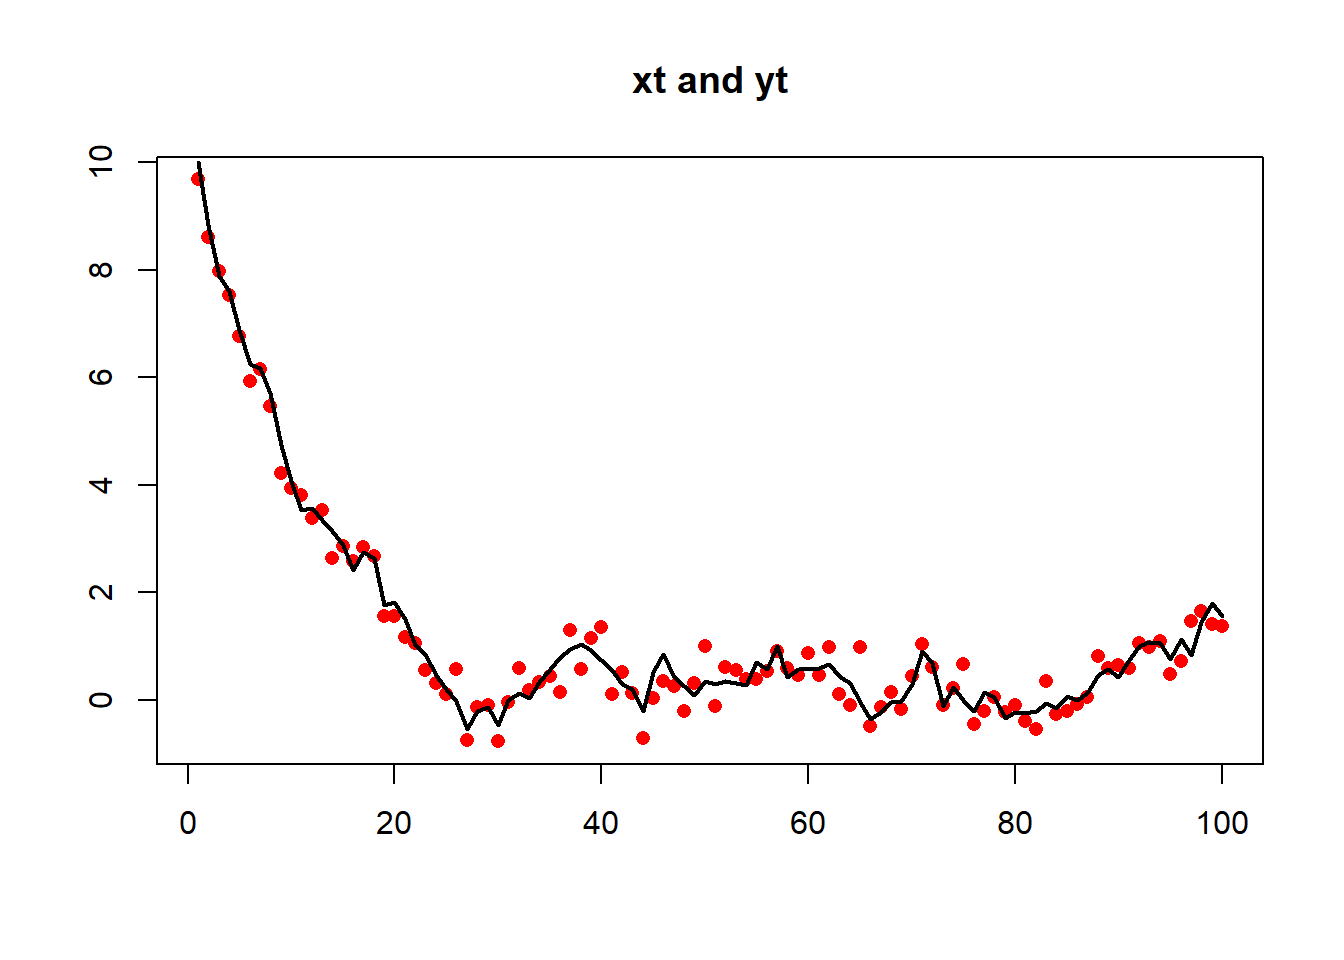
\includegraphics[width=0.8\linewidth]{MARSS_Manual_files/figure-latex/quick-unis-ar1-plot-1} \end{center}

\begin{Shaded}
\begin{Highlighting}[]
\NormalTok{fit <-}\StringTok{ }\KeywordTok{MARSS}\NormalTok{(yt.ns, }\DataTypeTok{model =} \KeywordTok{list}\NormalTok{(}\DataTypeTok{B =} \KeywordTok{matrix}\NormalTok{(}\StringTok{"b"}\NormalTok{)))}
\end{Highlighting}
\end{Shaded}

\begin{verbatim}
Success! abstol and log-log tests passed at 24 iterations.
Alert: conv.test.slope.tol is 0.5.
Test with smaller values (<0.1) to ensure convergence.

MARSS fit is
Estimation method: kem 
Convergence test: conv.test.slope.tol = 0.5, abstol = 0.001
Estimation converged in 24 iterations. 
Log-likelihood: -61.67475 
AIC: 133.3495   AICc: 133.9878   
 
      Estimate
R.R     0.1075
B.b     0.9042
U.U     0.0346
Q.Q     0.0535
x0.x0  10.6409
Initial states (x0) defined at t=0

Standard errors have not been calculated. 
Use MARSSparamCIs to compute CIs and bias estimates.
\end{verbatim}

We could also simulate AR(1) data with \texttt{stats::arima.sim()} however this will produce stationary data:

\begin{Shaded}
\begin{Highlighting}[]
\NormalTok{xt.s <-}\StringTok{ }\KeywordTok{arima.sim}\NormalTok{(}\DataTypeTok{n =}\NormalTok{ TT, }\DataTypeTok{model =} \KeywordTok{list}\NormalTok{(}\DataTypeTok{ar =}\NormalTok{ b), }\DataTypeTok{sd =} \KeywordTok{sqrt}\NormalTok{(q))}
\NormalTok{yt.s <-}\StringTok{ }\NormalTok{xt.s }\OperatorTok{+}\StringTok{ }\KeywordTok{rnorm}\NormalTok{(TT, }\DecValTok{0}\NormalTok{, }\KeywordTok{sqrt}\NormalTok{(r))}
\NormalTok{yt.s <-}\StringTok{ }\KeywordTok{as.vector}\NormalTok{(yt.s)}
\NormalTok{xt.s <-}\StringTok{ }\KeywordTok{as.vector}\NormalTok{(xt.s)}
\end{Highlighting}
\end{Shaded}

These stationary data can be fit as before but the data must be a matrix with time across the columns not a \textbf{ts} object. If you pass in a vector, \texttt{MARSS()} will convert that to a matrix with one row.

\begin{Shaded}
\begin{Highlighting}[]
\KeywordTok{plot}\NormalTok{(yt.s, }\DataTypeTok{xlab =} \StringTok{""}\NormalTok{, }\DataTypeTok{ylab =} \StringTok{""}\NormalTok{, }\DataTypeTok{main =} \StringTok{"xt and yt"}\NormalTok{, }\DataTypeTok{pch =} \DecValTok{16}\NormalTok{, }
    \DataTypeTok{col =} \StringTok{"red"}\NormalTok{, }\DataTypeTok{type =} \StringTok{"p"}\NormalTok{)}
\KeywordTok{lines}\NormalTok{(xt.s, }\DataTypeTok{lwd =} \DecValTok{2}\NormalTok{)}
\end{Highlighting}
\end{Shaded}

\begin{center}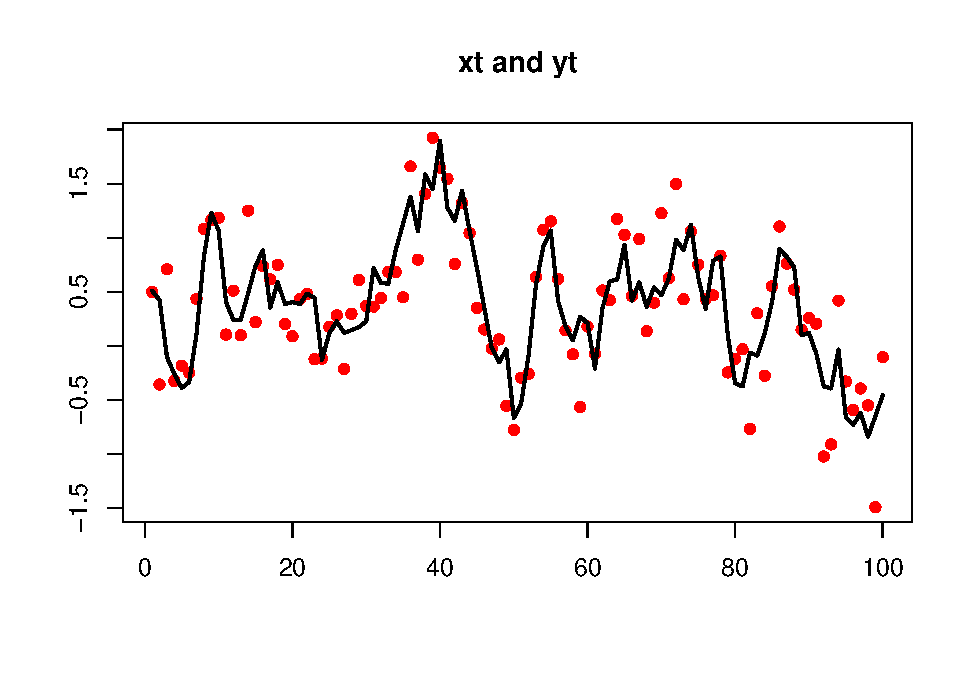
\includegraphics[width=0.8\linewidth]{MARSS_Manual_files/figure-latex/quick-unis-ar1-plot2-1} \end{center}

\begin{Shaded}
\begin{Highlighting}[]
\NormalTok{fit <-}\StringTok{ }\KeywordTok{MARSS}\NormalTok{(yt.s, }\DataTypeTok{model =} \KeywordTok{list}\NormalTok{(}\DataTypeTok{B =} \KeywordTok{matrix}\NormalTok{(}\StringTok{"b"}\NormalTok{)))}
\end{Highlighting}
\end{Shaded}

\begin{verbatim}
Success! abstol and log-log tests passed at 27 iterations.
Alert: conv.test.slope.tol is 0.5.
Test with smaller values (<0.1) to ensure convergence.

MARSS fit is
Estimation method: kem 
Convergence test: conv.test.slope.tol = 0.5, abstol = 0.001
Estimation converged in 27 iterations. 
Log-likelihood: -74.40797 
AIC: 158.8159   AICc: 159.4542   
 
      Estimate
R.R     0.1064
B.b     0.7884
U.U     0.0735
Q.Q     0.1142
x0.x0   0.2825
Initial states (x0) defined at t=0

Standard errors have not been calculated. 
Use MARSSparamCIs to compute CIs and bias estimates.
\end{verbatim}

Note that \(u\) is estimated however \texttt{arima.sim()} does not include a \(u\). We can set \(u\) to zero if we happened to know that it was zero.

\begin{Shaded}
\begin{Highlighting}[]
\NormalTok{fit <-}\StringTok{ }\KeywordTok{MARSS}\NormalTok{(yt.s, }\DataTypeTok{model =} \KeywordTok{list}\NormalTok{(}\DataTypeTok{B =} \KeywordTok{matrix}\NormalTok{(}\StringTok{"b"}\NormalTok{), }\DataTypeTok{U =} \KeywordTok{matrix}\NormalTok{(}\DecValTok{0}\NormalTok{)))}
\end{Highlighting}
\end{Shaded}

\begin{verbatim}
Success! abstol and log-log tests passed at 16 iterations.
Alert: conv.test.slope.tol is 0.5.
Test with smaller values (<0.1) to ensure convergence.

MARSS fit is
Estimation method: kem 
Convergence test: conv.test.slope.tol = 0.5, abstol = 0.001
Estimation converged in 16 iterations. 
Log-likelihood: -75.80277 
AIC: 159.6055   AICc: 160.0266   
 
      Estimate
R.R      0.117
B.b      0.874
Q.Q      0.100
x0.x0    0.339
Initial states (x0) defined at t=0

Standard errors have not been calculated. 
Use MARSSparamCIs to compute CIs and bias estimates.
\end{verbatim}

If we know \(r\) (or \(q\)), we could set those too:

\begin{Shaded}
\begin{Highlighting}[]
\NormalTok{fit <-}\StringTok{ }\KeywordTok{MARSS}\NormalTok{(yt.s, }\DataTypeTok{model =} \KeywordTok{list}\NormalTok{(}\DataTypeTok{B =} \KeywordTok{matrix}\NormalTok{(}\StringTok{"b"}\NormalTok{), }\DataTypeTok{U =} \KeywordTok{matrix}\NormalTok{(}\DecValTok{0}\NormalTok{), }
    \DataTypeTok{R =} \KeywordTok{matrix}\NormalTok{(r)))}
\end{Highlighting}
\end{Shaded}

\begin{verbatim}
Success! abstol and log-log tests passed at 18 iterations.
Alert: conv.test.slope.tol is 0.5.
Test with smaller values (<0.1) to ensure convergence.

MARSS fit is
Estimation method: kem 
Convergence test: conv.test.slope.tol = 0.5, abstol = 0.001
Estimation converged in 18 iterations. 
Log-likelihood: -75.88583 
AIC: 157.7717   AICc: 158.0217   
 
      Estimate
B.b      0.859
Q.Q      0.114
x0.x0    0.370
Initial states (x0) defined at t=0

Standard errors have not been calculated. 
Use MARSSparamCIs to compute CIs and bias estimates.
\end{verbatim}

We can fit to just the \(x\) data, an AR(1) with no error, by setting \(r\) to zero:
If we know \(r\) (or \(q\)), we could set those too:

\begin{Shaded}
\begin{Highlighting}[]
\NormalTok{fit <-}\StringTok{ }\KeywordTok{MARSS}\NormalTok{(xt.s, }\DataTypeTok{model =} \KeywordTok{list}\NormalTok{(}\DataTypeTok{B =} \KeywordTok{matrix}\NormalTok{(}\StringTok{"b"}\NormalTok{), }\DataTypeTok{U =} \KeywordTok{matrix}\NormalTok{(}\DecValTok{0}\NormalTok{), }
    \DataTypeTok{R =} \KeywordTok{matrix}\NormalTok{(}\DecValTok{0}\NormalTok{)))}
\end{Highlighting}
\end{Shaded}

\begin{verbatim}
Success! algorithm run for 15 iterations. abstol and log-log tests passed.
Alert: conv.test.slope.tol is 0.5.
Test with smaller values (<0.1) to ensure convergence.

MARSS fit is
Estimation method: kem 
Convergence test: conv.test.slope.tol = 0.5, abstol = 0.001
Algorithm ran 15 (=minit) iterations and convergence was reached. 
Log-likelihood: -26.9401 
AIC: 59.8802   AICc: 60.1302   
 
      Estimate
B.b      0.883
Q.Q      0.100
x0.x0    0.578
Initial states (x0) defined at t=0

Standard errors have not been calculated. 
Use MARSSparamCIs to compute CIs and bias estimates.
\end{verbatim}

We can fit \texttt{xt.s} with \texttt{arima()} also. The results will be similar but not identical because \texttt{arima()}'s algorithm assumes the data come from a stationary process and the initial conditions are treated differently.

\begin{Shaded}
\begin{Highlighting}[]
\KeywordTok{arima}\NormalTok{(xt.s, }\DataTypeTok{order =} \KeywordTok{c}\NormalTok{(}\DecValTok{1}\NormalTok{, }\DecValTok{0}\NormalTok{, }\DecValTok{0}\NormalTok{), }\DataTypeTok{include.mean =} \OtherTok{FALSE}\NormalTok{, }\DataTypeTok{method =} \StringTok{"ML"}\NormalTok{)}
\end{Highlighting}
\end{Shaded}

\begin{verbatim}

Call:
arima(x = xt.s, order = c(1, 0, 0), include.mean = FALSE, method = "ML")

Coefficients:
         ar1
      0.8793
s.e.  0.0454

sigma^2 estimated as 0.1009:  log likelihood = -27.98,  aic = 59.96
\end{verbatim}

If we try fitting the non-stationary data with \texttt{arima()}, the estimates will be poor since \texttt{arima()} assumes stationary data:

\begin{Shaded}
\begin{Highlighting}[]
\KeywordTok{arima}\NormalTok{(xt.ns, }\DataTypeTok{order =} \KeywordTok{c}\NormalTok{(}\DecValTok{1}\NormalTok{, }\DecValTok{0}\NormalTok{, }\DecValTok{0}\NormalTok{), }\DataTypeTok{include.mean =} \OtherTok{FALSE}\NormalTok{, }\DataTypeTok{method =} \StringTok{"ML"}\NormalTok{)}
\end{Highlighting}
\end{Shaded}

\begin{verbatim}

Call:
arima(x = xt.ns, order = c(1, 0, 0), include.mean = FALSE, method = "ML")

Coefficients:
         ar1
      0.9985
s.e.  0.0021

sigma^2 estimated as 0.1348:  log likelihood = -44.59,  aic = 93.19
\end{verbatim}

\hypertarget{linear-regression-with-ar1-errors}{%
\section{Linear regression with AR(1) errors}\label{linear-regression-with-ar1-errors}}

A simple linear regression of one covariate with AR(1) errors is written:

\begin{gather}
x_{t} = bx_{t-1} + w_{t}, \text{ } w_t \sim \,\text{N}(0,q)  \\
y_{t} = \beta*d_t + x_{t}
(\#eq:short.lr.ar1)
\end{gather}

Let's create some simulated data with this structure:

\begin{Shaded}
\begin{Highlighting}[]
\NormalTok{beta <-}\StringTok{ }\FloatTok{1.1}
\NormalTok{dt <-}\StringTok{ }\KeywordTok{rnorm}\NormalTok{(TT, }\DecValTok{0}\NormalTok{, }\DecValTok{1}\NormalTok{)  }\CommentTok{#our covariate}
\NormalTok{wt <-}\StringTok{ }\KeywordTok{arima.sim}\NormalTok{(}\DataTypeTok{n =}\NormalTok{ TT, }\DataTypeTok{model =} \KeywordTok{list}\NormalTok{(}\DataTypeTok{ar =}\NormalTok{ b), }\DataTypeTok{sd =} \KeywordTok{sqrt}\NormalTok{(q))}
\NormalTok{yt <-}\StringTok{ }\NormalTok{beta }\OperatorTok{*}\StringTok{ }\NormalTok{dt }\OperatorTok{+}\StringTok{ }\NormalTok{wt}
\NormalTok{yt <-}\StringTok{ }\KeywordTok{as.vector}\NormalTok{(yt)  }\CommentTok{# not ts object}
\KeywordTok{plot}\NormalTok{(dt, yt)}
\end{Highlighting}
\end{Shaded}

\begin{center}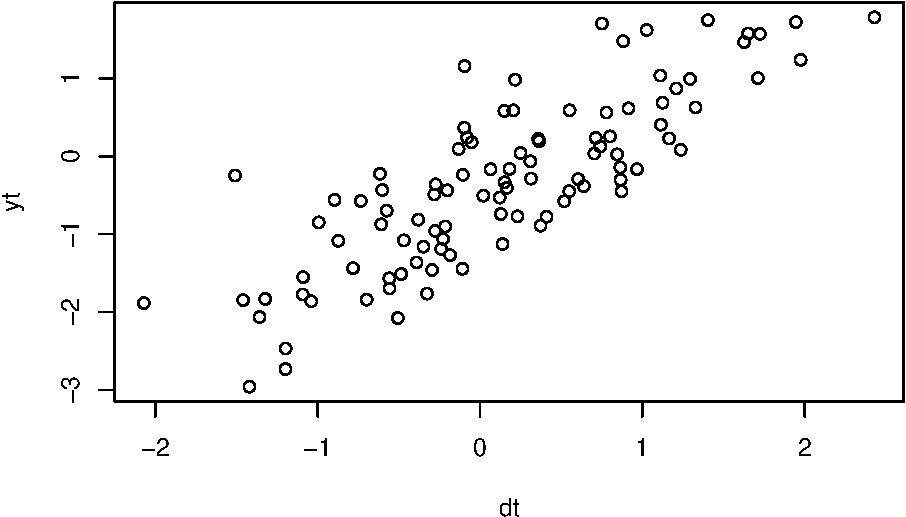
\includegraphics[width=0.8\linewidth]{MARSS_Manual_files/figure-latex/quick-unis-lm-ar1-1} \end{center}

If we looked at an ACF of the residuals of a linear regression, we'd see that the residuals are highly autocorrelated:

\begin{Shaded}
\begin{Highlighting}[]
\KeywordTok{acf}\NormalTok{(}\KeywordTok{residuals}\NormalTok{(}\KeywordTok{lm}\NormalTok{(yt }\OperatorTok{~}\StringTok{ }\NormalTok{dt)))}
\end{Highlighting}
\end{Shaded}

\begin{center}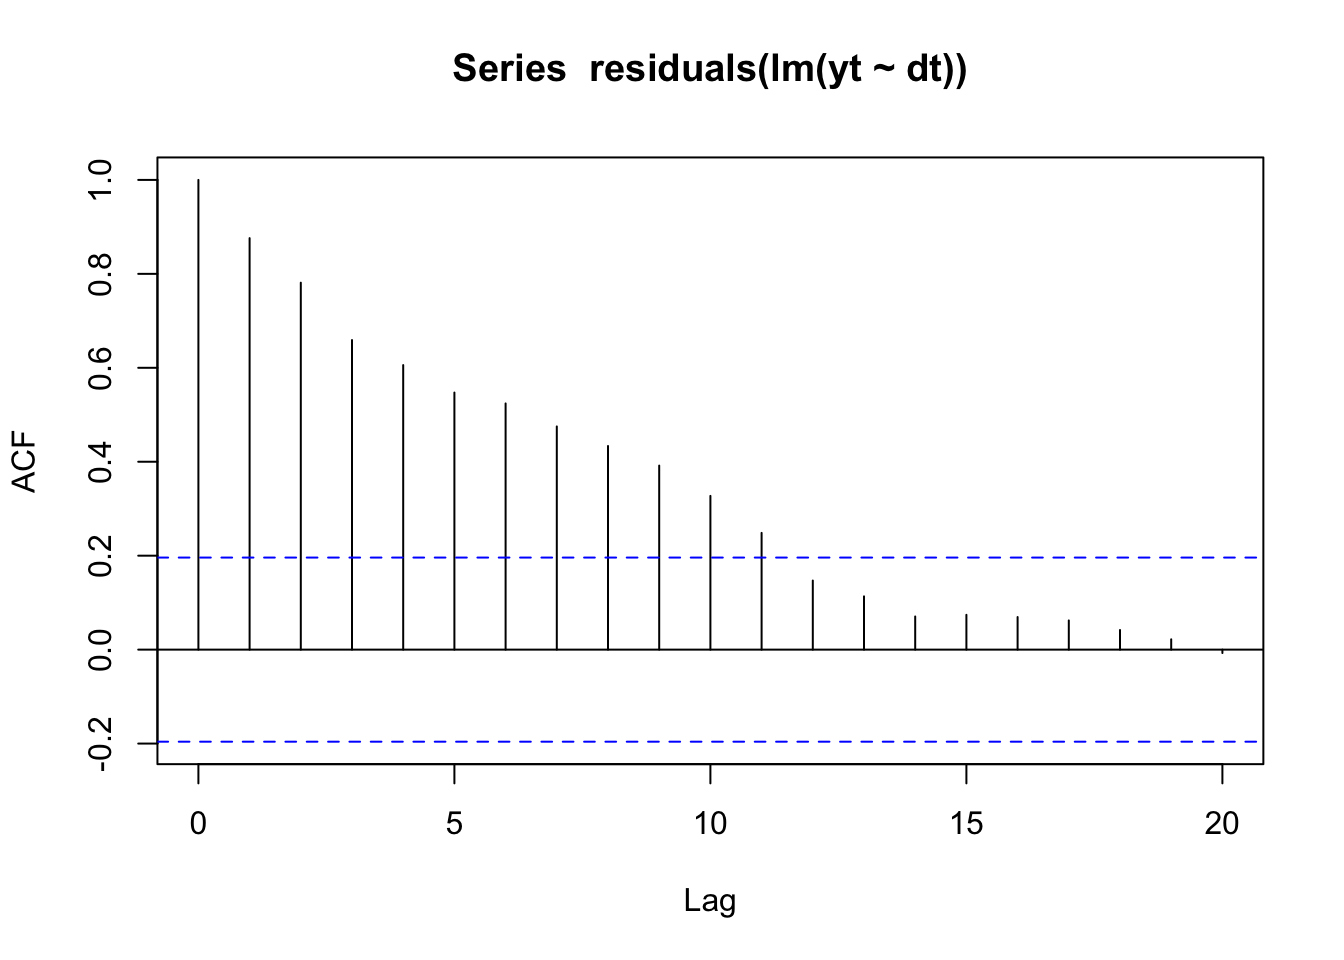
\includegraphics[width=0.8\linewidth]{MARSS_Manual_files/figure-latex/quick-unis-lm-ar1-acf-1} \end{center}

We can fit this model (Equation @ref(eq:short.lr.ar1)) with \texttt{MARSS()}. Please note that there are many better ,\textbf{R} packages specifically designed for linear regression models with correlated errors. This simple example is to help you understand model specification with the \textbf{MARSS} package.

To fit this model, we need match our Equation @ref(eq:short.lr.ar1) with the full MARSS model written in matrix form (Equation @ref(eq:marss.part2)). Here it is with the parameters that are zero dropped. \(\mathbf{Z}_t\) is identity and is also dropped. The \(\mathbf{B}\) and \(\mathbf{D}\) are time-constant so the \(t\) subscript is dropped. The \(\mathbf{x}_t\) are the AR(1) errors and the \(\mathbf{y}_t\) is the linear regression with \(\mathbf{D}\) being the effect sizes and the \(\mathbf{d}\) being the covariate.

\begin{equation}(\#eq:short.lr.ar1.marss)
\begin{gather}
\mathbf{x}_t = \mathbf{B}\mathbf{x}_{t-1} + \mathbf{w}_t, \text{ where } \mathbf{w}_t \sim \,\text{MVN}(0,\mathbf{Q}_t)\\
\mathbf{y}_t = \mathbf{x}_t + \mathbf{D}\mathbf{d}_t
\end{gather}
\end{equation}

Here is what the model looks like if we write the parameters explicitly in matrix form. The matrices are \(1 \times 1\).
\begin{gather}
\begin{bmatrix}x\end{bmatrix}_{t} = \begin{bmatrix}b\end{bmatrix}\begin{bmatrix}x\end{bmatrix}_{t-1} + \begin{bmatrix}0\end{bmatrix} + \begin{bmatrix}w\end{bmatrix}_{t}  \\
\begin{bmatrix}y\end{bmatrix}_{t} = \begin{bmatrix}x\end{bmatrix}_{t} + \begin{bmatrix}\beta\end{bmatrix}\begin{bmatrix}d\end{bmatrix}_t
(\#eq:short.lr.ar1.mat)
\end{gather}

To create the model list for \texttt{MARSS()}, we specify the parameter matrices one-to-one like they look in Equation @ref(eq:short.lr.ar1.mat).

\begin{Shaded}
\begin{Highlighting}[]
\NormalTok{R <-}\StringTok{ }\KeywordTok{matrix}\NormalTok{(}\StringTok{"r"}\NormalTok{)  }\CommentTok{# no v_t}
\NormalTok{D <-}\StringTok{ }\KeywordTok{matrix}\NormalTok{(}\StringTok{"beta"}\NormalTok{)}
\NormalTok{U <-}\StringTok{ }\KeywordTok{matrix}\NormalTok{(}\DecValTok{0}\NormalTok{)  }\CommentTok{# since arima.sim was used, no u}
\NormalTok{B <-}\StringTok{ }\KeywordTok{matrix}\NormalTok{(}\StringTok{"b"}\NormalTok{)}
\NormalTok{d <-}\StringTok{ }\KeywordTok{matrix}\NormalTok{(dt, }\DataTypeTok{nrow =} \DecValTok{1}\NormalTok{)}
\NormalTok{A <-}\StringTok{ }\KeywordTok{matrix}\NormalTok{(}\DecValTok{0}\NormalTok{)}
\end{Highlighting}
\end{Shaded}

\texttt{MARSS()} requires \(\mathbf{d}\) be a matrix also. Each row is a covariate and each column is a time step. No missing values allowed as this is an input.

How should we treat the \(\mathbf{R}\) matrix? It is zero, and we could set \(\mathbf{R}\) to zero:

\begin{verbatim}
R <- matrix(0)
\end{verbatim}

However, the EM algorithm in the \textbf{MARSS} package will not perform well at all with \(\mathbf{R}\) set to zero and it has to do with how \(\mathbf{R}=0\) affects the update equations. You can use the BFGS algorithm or estimate \(\mathbf{R}\).

\begin{Shaded}
\begin{Highlighting}[]
\NormalTok{R <-}\StringTok{ }\KeywordTok{matrix}\NormalTok{(}\StringTok{"r"}\NormalTok{)}
\NormalTok{mod.list <-}\StringTok{ }\KeywordTok{list}\NormalTok{(}\DataTypeTok{B =}\NormalTok{ B, }\DataTypeTok{U =}\NormalTok{ U, }\DataTypeTok{R =}\NormalTok{ R, }\DataTypeTok{D =}\NormalTok{ D, }\DataTypeTok{d =}\NormalTok{ d, }\DataTypeTok{A =}\NormalTok{ A)}
\NormalTok{fit <-}\StringTok{ }\KeywordTok{MARSS}\NormalTok{(yt, }\DataTypeTok{model =}\NormalTok{ mod.list)}
\end{Highlighting}
\end{Shaded}

\begin{verbatim}
Warning! Abstol convergence only. Maxit (=500) reached before log-log convergence.

MARSS fit is
Estimation method: kem 
Convergence test: conv.test.slope.tol = 0.5, abstol = 0.001
WARNING: Abstol convergence only no log-log convergence.
 maxit (=500) reached before log-log convergence.
 The likelihood and params might not be at the ML values.
 Try setting control$maxit higher.
Log-likelihood: -25.53381 
AIC: 61.06762   AICc: 61.70592   
 
       Estimate
R.r     0.00264
B.b     0.91256
Q.Q     0.09294
x0.x0  -1.07486
D.beta  1.10169
Initial states (x0) defined at t=0

Standard errors have not been calculated. 
Use MARSSparamCIs to compute CIs and bias estimates.

Convergence warnings
 Warning: the  R.r  parameter value has not converged.
 Type MARSSinfo("convergence") for more info on this warning.
\end{verbatim}

Or use the BFGS algorithm for fitting:

\begin{Shaded}
\begin{Highlighting}[]
\NormalTok{R <-}\StringTok{ }\KeywordTok{matrix}\NormalTok{(}\DecValTok{0}\NormalTok{)}
\NormalTok{mod.list <-}\StringTok{ }\KeywordTok{list}\NormalTok{(}\DataTypeTok{B =}\NormalTok{ B, }\DataTypeTok{U =}\NormalTok{ U, }\DataTypeTok{R =}\NormalTok{ R, }\DataTypeTok{D =}\NormalTok{ D, }\DataTypeTok{d =}\NormalTok{ d, }\DataTypeTok{A =}\NormalTok{ A)}
\NormalTok{fit <-}\StringTok{ }\KeywordTok{MARSS}\NormalTok{(yt, }\DataTypeTok{model =}\NormalTok{ mod.list, }\DataTypeTok{method =} \StringTok{"BFGS"}\NormalTok{)}
\end{Highlighting}
\end{Shaded}

\begin{verbatim}
Success! Converged in 122 iterations.
Function MARSSkfas used for likelihood calculation.

MARSS fit is
Estimation method: BFGS 
Estimation converged in 122 iterations. 
Log-likelihood: -25.48386 
AIC: 58.96772   AICc: 59.38878   
 
       Estimate
B.b      0.9090
Q.Q      0.0975
x0.x0   -1.0754
D.beta   1.1017
Initial states (x0) defined at t=0

Standard errors have not been calculated. 
Use MARSSparamCIs to compute CIs and bias estimates.
\end{verbatim}

This is the same model you are fitting when you pass in \texttt{xreg} with the \texttt{arima()} function:

\begin{Shaded}
\begin{Highlighting}[]
\NormalTok{stats}\OperatorTok{::}\KeywordTok{arima}\NormalTok{(yt, }\DataTypeTok{order =} \KeywordTok{c}\NormalTok{(}\DecValTok{1}\NormalTok{, }\DecValTok{0}\NormalTok{, }\DecValTok{0}\NormalTok{), }\DataTypeTok{xreg =}\NormalTok{ dt, }\DataTypeTok{include.mean =} \OtherTok{FALSE}\NormalTok{, }
    \DataTypeTok{method =} \StringTok{"ML"}\NormalTok{)}
\end{Highlighting}
\end{Shaded}

\begin{verbatim}

Call:
stats::arima(x = yt, order = c(1, 0, 0), xreg = dt, include.mean = FALSE, method = "ML")

Coefficients:
         ar1      dt
      0.9143  1.1023
s.e.  0.0384  0.0266

sigma^2 estimated as 0.09906:  log likelihood = -27.19,  aic = 60.39
\end{verbatim}

Again the estimates are slightly different due to different treatment of the initial conditons.

\hypertarget{linear-regression-with-ar1-errors-and-independent-errors}{%
\section{Linear regression with AR(1) errors and independent errors}\label{linear-regression-with-ar1-errors-and-independent-errors}}

We can add some independent error to our model:

\begin{gather}
x_{t} = bx_{t-1} + w_{t}, \text{ } w_t \sim \,\text{N}(0,q)  \\
y_{t} = \beta*d_t + x_{t} + v_t, , \text{ } v_t \sim \,\text{N}(0,r)  
(\#eq:short.lr.ar1.r)
\end{gather}

We'll generate this data by adding independent error to \texttt{yt} from the previous example.

\begin{Shaded}
\begin{Highlighting}[]
\NormalTok{yt.r <-}\StringTok{ }\NormalTok{yt }\OperatorTok{+}\StringTok{ }\KeywordTok{rnorm}\NormalTok{(TT, }\DecValTok{0}\NormalTok{, }\KeywordTok{sqrt}\NormalTok{(r))}
\end{Highlighting}
\end{Shaded}

We can fit as:

\begin{Shaded}
\begin{Highlighting}[]
\NormalTok{R <-}\StringTok{ }\KeywordTok{matrix}\NormalTok{(}\StringTok{"r"}\NormalTok{)}
\NormalTok{mod.list <-}\StringTok{ }\KeywordTok{list}\NormalTok{(}\DataTypeTok{B =}\NormalTok{ B, }\DataTypeTok{U =}\NormalTok{ U, }\DataTypeTok{R =}\NormalTok{ R, }\DataTypeTok{D =}\NormalTok{ D, }\DataTypeTok{d =}\NormalTok{ d, }\DataTypeTok{A =}\NormalTok{ A)}
\NormalTok{fit <-}\StringTok{ }\KeywordTok{MARSS}\NormalTok{(yt.r, }\DataTypeTok{model =}\NormalTok{ mod.list)}
\end{Highlighting}
\end{Shaded}

\begin{verbatim}
Success! abstol and log-log tests passed at 30 iterations.
Alert: conv.test.slope.tol is 0.5.
Test with smaller values (<0.1) to ensure convergence.

MARSS fit is
Estimation method: kem 
Convergence test: conv.test.slope.tol = 0.5, abstol = 0.001
Estimation converged in 30 iterations. 
Log-likelihood: -71.13411 
AIC: 152.2682   AICc: 152.9065   
 
       Estimate
R.r      0.1172
B.b      0.9259
Q.Q      0.0747
x0.x0   -0.8778
D.beta   1.0974
Initial states (x0) defined at t=0

Standard errors have not been calculated. 
Use MARSSparamCIs to compute CIs and bias estimates.
\end{verbatim}

This is not a model that can be fit with \texttt{arima()}.

\hypertarget{linear-regression-with-ar1-driven-by-covariate}{%
\section{Linear regression with AR(1) driven by covariate}\label{linear-regression-with-ar1-driven-by-covariate}}

We can model a situation where the regression errors are autocorrelated but some of the variance is driven by a covariate. For example, good and bad `years' are driven partially by, say, temperature, which we will model by \texttt{ct}. We will use an autocorrelated \texttt{ct} in the example, but it could be anything. How are autocorrelated errors different? There is memory in the errors. The \texttt{ct} in the past still affects the current error (\(w_t\) in this model).

\begin{gather}
x_{t} = bx_{t-1} + \beta*c_t + w_{t}, \text{ } w_t \sim \,\text{N}(0,q)  \\
y_{t} = x_{t} + v_t, \text{ } v_t \sim \,\text{N}(0,r)  
(\#eq:short.lr.ar1.c)
\end{gather}

Let's create some simulated data with this structure:

\begin{Shaded}
\begin{Highlighting}[]
\NormalTok{beta <-}\StringTok{ }\FloatTok{1.1}
\NormalTok{x0 <-}\StringTok{ }\DecValTok{0}
\NormalTok{ct <-}\StringTok{ }\KeywordTok{arima.sim}\NormalTok{(}\DataTypeTok{n =}\NormalTok{ TT, }\DataTypeTok{model =} \KeywordTok{list}\NormalTok{(}\DataTypeTok{ar =} \FloatTok{0.8}\NormalTok{), }\DataTypeTok{sd =} \KeywordTok{sqrt}\NormalTok{(}\DecValTok{1}\NormalTok{))  }\CommentTok{# our covariate}
\NormalTok{ct <-}\StringTok{ }\KeywordTok{as.vector}\NormalTok{(ct)}
\NormalTok{xt <-}\StringTok{ }\KeywordTok{rep}\NormalTok{(x0, TT)}
\ControlFlowTok{for}\NormalTok{ (i }\ControlFlowTok{in} \DecValTok{2}\OperatorTok{:}\NormalTok{TT) xt[i] <-}\StringTok{ }\NormalTok{b }\OperatorTok{*}\StringTok{ }\NormalTok{xt[i }\OperatorTok{-}\StringTok{ }\DecValTok{1}\NormalTok{] }\OperatorTok{+}\StringTok{ }\NormalTok{beta }\OperatorTok{*}\StringTok{ }\NormalTok{ct[i] }\OperatorTok{+}\StringTok{ }\KeywordTok{rnorm}\NormalTok{(}\DecValTok{1}\NormalTok{, }
    \DecValTok{0}\NormalTok{, }\KeywordTok{sqrt}\NormalTok{(q))}
\NormalTok{yt <-}\StringTok{ }\NormalTok{xt }\OperatorTok{+}\StringTok{ }\KeywordTok{rnorm}\NormalTok{(TT, }\DecValTok{0}\NormalTok{, }\KeywordTok{sqrt}\NormalTok{(r))}
\end{Highlighting}
\end{Shaded}

To fit this with \texttt{MARSS()}, we match up the model to the full MARSS model form:

\begin{equation}
\begin{gather}
\mathbf{x}_t = \mathbf{B}\mathbf{x}_{t-1} + \mathbf{C}\mathbf{c}_t + \mathbf{w}_t, \text{ where } \mathbf{w}_t \sim \,\text{MVN}(0,\mathbf{Q}_t)\\
\mathbf{y}_t = \mathbf{x}_t + \mathbf{v}_t, \text{ where } \mathbf{v}_t \sim \,\text{MVN}(0,\mathbf{R}_t)
\end{gather}
\end{equation}

The model list for \texttt{MARSS()} is:

\begin{Shaded}
\begin{Highlighting}[]
\NormalTok{R <-}\StringTok{ }\KeywordTok{matrix}\NormalTok{(}\StringTok{"r"}\NormalTok{)  }\CommentTok{# no v_t}
\NormalTok{C <-}\StringTok{ }\KeywordTok{matrix}\NormalTok{(}\StringTok{"beta"}\NormalTok{)}
\NormalTok{U <-}\StringTok{ }\KeywordTok{matrix}\NormalTok{(}\DecValTok{0}\NormalTok{)  }\CommentTok{# no u}
\NormalTok{B <-}\StringTok{ }\KeywordTok{matrix}\NormalTok{(}\StringTok{"b"}\NormalTok{)}
\NormalTok{c <-}\StringTok{ }\KeywordTok{matrix}\NormalTok{(ct, }\DataTypeTok{nrow =} \DecValTok{1}\NormalTok{)}
\NormalTok{A <-}\StringTok{ }\KeywordTok{matrix}\NormalTok{(}\DecValTok{0}\NormalTok{)}
\end{Highlighting}
\end{Shaded}

Now fit:

\begin{Shaded}
\begin{Highlighting}[]
\NormalTok{mod.list <-}\StringTok{ }\KeywordTok{list}\NormalTok{(}\DataTypeTok{B =}\NormalTok{ B, }\DataTypeTok{U =}\NormalTok{ U, }\DataTypeTok{R =}\NormalTok{ R, }\DataTypeTok{C =}\NormalTok{ C, }\DataTypeTok{c =}\NormalTok{ c, }\DataTypeTok{A =}\NormalTok{ A)}
\NormalTok{fit <-}\StringTok{ }\KeywordTok{MARSS}\NormalTok{(yt, }\DataTypeTok{model =}\NormalTok{ mod.list)}
\end{Highlighting}
\end{Shaded}

\begin{verbatim}
Success! abstol and log-log tests passed at 18 iterations.
Alert: conv.test.slope.tol is 0.5.
Test with smaller values (<0.1) to ensure convergence.

MARSS fit is
Estimation method: kem 
Convergence test: conv.test.slope.tol = 0.5, abstol = 0.001
Estimation converged in 18 iterations. 
Log-likelihood: -79.55739 
AIC: 169.1148   AICc: 169.7531   
 
       Estimate
R.r       0.100
B.b       0.900
Q.Q       0.135
x0.x0    -1.006
C.beta    1.120
Initial states (x0) defined at t=0

Standard errors have not been calculated. 
Use MARSSparamCIs to compute CIs and bias estimates.
\end{verbatim}

\hypertarget{flat-level-model}{%
\section{Flat level model}\label{flat-level-model}}

For the next examples, we will use the Nile river flow from 1871 to 1970, a data set in the \textbf{datasets} package.

\begin{Shaded}
\begin{Highlighting}[]
\NormalTok{nile <-}\StringTok{ }\KeywordTok{as.vector}\NormalTok{(datasets}\OperatorTok{::}\NormalTok{Nile)}
\NormalTok{year <-}\StringTok{ }\KeywordTok{as.vector}\NormalTok{(}\KeywordTok{time}\NormalTok{(Nile))}
\end{Highlighting}
\end{Shaded}

The first model we will fit is a flat level model:

\begin{equation}
y_t = a+v_t, \text{ } v_t \sim \,\text{N}(0,r)    
(\#eq:short.flat.level)
\end{equation}
where \(y_t\) is the river flow volume at year \(t\) and \(a\) is some constant average flow level (notice it has no \(t\) subscript).

To fit this model with MARSS, we explicitly show all the MARSS parameters.
\begin{equation}
\begin{gathered}
x_t = 1 \times x_{t-1}+ 0 + w_t,    \text{ } w_t \sim \,\text{N}(0,0) \\
y_t = 0 \times x_t + a + v_t, \text{ } v_t \sim \,\text{N}(0,r)  \\
x_0 = 0 
 \end{gathered}   
(\#eq:short.flat.level.model1)
\end{equation}

The model list and fit for this equation is

\begin{Shaded}
\begin{Highlighting}[]
\NormalTok{mod.list1 <-}\StringTok{ }\KeywordTok{list}\NormalTok{(}\DataTypeTok{Z =} \KeywordTok{matrix}\NormalTok{(}\DecValTok{0}\NormalTok{), }\DataTypeTok{A =} \KeywordTok{matrix}\NormalTok{(}\StringTok{"a"}\NormalTok{), }\DataTypeTok{R =} \KeywordTok{matrix}\NormalTok{(}\StringTok{"r"}\NormalTok{), }
    \DataTypeTok{B =} \KeywordTok{matrix}\NormalTok{(}\DecValTok{1}\NormalTok{), }\DataTypeTok{U =} \KeywordTok{matrix}\NormalTok{(}\DecValTok{0}\NormalTok{), }\DataTypeTok{Q =} \KeywordTok{matrix}\NormalTok{(}\DecValTok{0}\NormalTok{), }\DataTypeTok{x0 =} \KeywordTok{matrix}\NormalTok{(}\DecValTok{0}\NormalTok{))}
\NormalTok{fit1 <-}\StringTok{ }\KeywordTok{MARSS}\NormalTok{(nile, }\DataTypeTok{model =}\NormalTok{ mod.list1)}
\end{Highlighting}
\end{Shaded}

\begin{verbatim}
Success! abstol and log-log tests passed at 16 iterations.
Alert: conv.test.slope.tol is 0.5.
Test with smaller values (<0.1) to ensure convergence.

MARSS fit is
Estimation method: kem 
Convergence test: conv.test.slope.tol = 0.5, abstol = 0.001
Estimation converged in 16 iterations. 
Log-likelihood: -654.5157 
AIC: 1313.031   AICc: 1313.155   
 
    Estimate
A.a      919
R.r    28352
Initial states (x0) defined at t=0

Standard errors have not been calculated. 
Use MARSSparamCIs to compute CIs and bias estimates.
\end{verbatim}

MARSS includes the state process \(x_t\) but we are setting \(\mathbf{Z}\) to zero so that \(x_t\) does not appear in our observation model. We need to fix all the state parameters to zero so that the algorithm doesn't ``chase its tail'' trying to fit \(x_t\) to the data.

An equivalent way to write this model is to use \(x_t\) as the average flow level and make it be a constant level by setting \(q=0\). The average flow appears as the \(x_0\) parameter. In MARSS form, this model is:

\begin{equation}
\begin{gathered}
x_t = 1 \times x_{t-1}+ 0 + w_t    \text{ where } w_t \sim \,\text{N}(0,0) \\
y_t = 1 \times x_t + 0 + v_t \text{ where } v_t \sim \,\text{N}(0,r)  \\
x_0 = a 
 \end{gathered}   
(\#eq:short.flat.level.model2)
\end{equation}

The model list and fit for this equation is

\begin{Shaded}
\begin{Highlighting}[]
\NormalTok{mod.list2 <-}\StringTok{ }\KeywordTok{list}\NormalTok{(}\DataTypeTok{Z =} \KeywordTok{matrix}\NormalTok{(}\DecValTok{1}\NormalTok{), }\DataTypeTok{A =} \KeywordTok{matrix}\NormalTok{(}\DecValTok{0}\NormalTok{), }\DataTypeTok{R =} \KeywordTok{matrix}\NormalTok{(}\StringTok{"r"}\NormalTok{), }
    \DataTypeTok{B =} \KeywordTok{matrix}\NormalTok{(}\DecValTok{1}\NormalTok{), }\DataTypeTok{U =} \KeywordTok{matrix}\NormalTok{(}\DecValTok{0}\NormalTok{), }\DataTypeTok{Q =} \KeywordTok{matrix}\NormalTok{(}\DecValTok{0}\NormalTok{), }\DataTypeTok{x0 =} \KeywordTok{matrix}\NormalTok{(}\StringTok{"a"}\NormalTok{))}
\NormalTok{fit2 <-}\StringTok{ }\KeywordTok{MARSS}\NormalTok{(nile, }\DataTypeTok{model =}\NormalTok{ mod.list2)}
\end{Highlighting}
\end{Shaded}

\begin{verbatim}
Success! algorithm run for 15 iterations. abstol and log-log tests passed.
Alert: conv.test.slope.tol is 0.5.
Test with smaller values (<0.1) to ensure convergence.

MARSS fit is
Estimation method: kem 
Convergence test: conv.test.slope.tol = 0.5, abstol = 0.001
Algorithm ran 15 (=minit) iterations and convergence was reached. 
Log-likelihood: -654.5157 
AIC: 1313.031   AICc: 1313.155   
 
     Estimate
R.r     28352
x0.a      919
Initial states (x0) defined at t=0

Standard errors have not been calculated. 
Use MARSSparamCIs to compute CIs and bias estimates.
\end{verbatim}

The results are the same. We just formatted the model in different ways. We can plot the fitted model against the Nile river flow (blue dots) using \texttt{autoplot()}.

\begin{Shaded}
\begin{Highlighting}[]
\NormalTok{ggplot2}\OperatorTok{::}\KeywordTok{autoplot}\NormalTok{(fit2, }\DataTypeTok{plot.type =} \StringTok{"observations"}\NormalTok{)}
\end{Highlighting}
\end{Shaded}

\begin{center}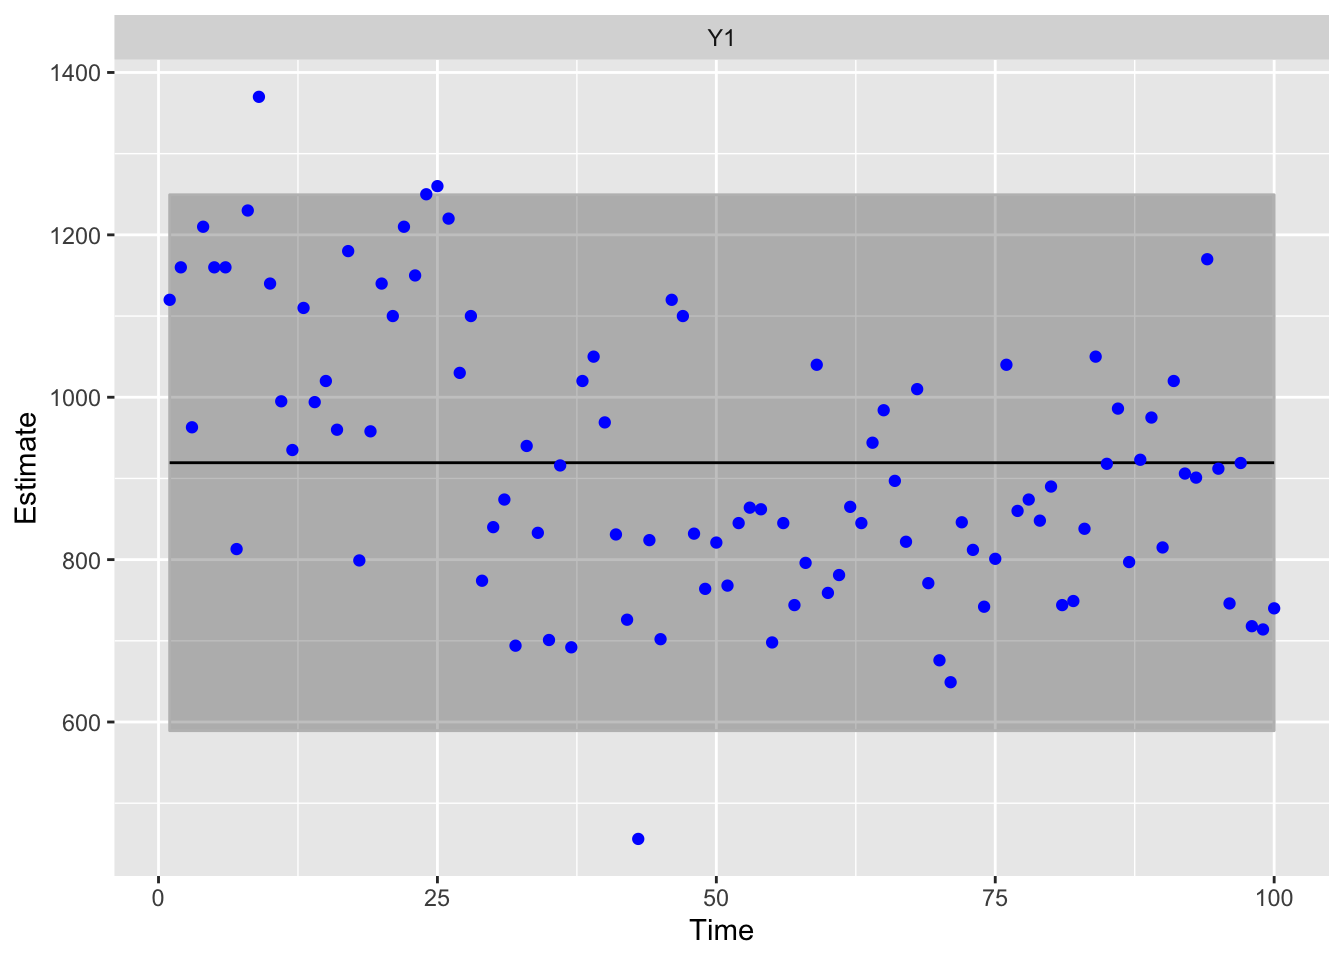
\includegraphics[width=0.8\linewidth]{MARSS_Manual_files/figure-latex/quick-unis-flat-level-plot-1} \end{center}

\hypertarget{linear-trend-model}{%
\section{Linear trend model}\label{linear-trend-model}}

Looking at the data, we might expect that a declining average river flow would be better. In MARSS form, that model would be:
\begin{equation}
\begin{gathered}
x_t = 1 \times x_{t-1}+ 0 + w_t,    \text{ } w_t \sim \,\text{N}(0,0) \\
y_t = 0 \times x_t + a + \beta*t + v_t, \text{ } v_t \sim \,\text{N}(0,r)  \\
x_0 = 0 
\end{gathered}   
(\#eq:short.linear.level.model1)
\end{equation}
where \(t\) is the year and \(u\) is the average per-year decline in river flow volume.

The model list and fit for this equation is

\begin{Shaded}
\begin{Highlighting}[]
\NormalTok{mod.list1 <-}\StringTok{ }\KeywordTok{list}\NormalTok{(}\DataTypeTok{Z =} \KeywordTok{matrix}\NormalTok{(}\DecValTok{0}\NormalTok{), }\DataTypeTok{A =} \KeywordTok{matrix}\NormalTok{(}\StringTok{"a"}\NormalTok{), }\DataTypeTok{R =} \KeywordTok{matrix}\NormalTok{(}\StringTok{"r"}\NormalTok{), }
    \DataTypeTok{D =} \KeywordTok{matrix}\NormalTok{(}\StringTok{"beta"}\NormalTok{), }\DataTypeTok{d =} \KeywordTok{matrix}\NormalTok{(}\DecValTok{1}\OperatorTok{:}\DecValTok{100}\NormalTok{, }\DataTypeTok{nrow =} \DecValTok{1}\NormalTok{), }\DataTypeTok{B =} \KeywordTok{matrix}\NormalTok{(}\DecValTok{1}\NormalTok{), }
    \DataTypeTok{U =} \KeywordTok{matrix}\NormalTok{(}\DecValTok{0}\NormalTok{), }\DataTypeTok{Q =} \KeywordTok{matrix}\NormalTok{(}\DecValTok{0}\NormalTok{), }\DataTypeTok{x0 =} \KeywordTok{matrix}\NormalTok{(}\DecValTok{0}\NormalTok{))}
\NormalTok{fit1 <-}\StringTok{ }\KeywordTok{MARSS}\NormalTok{(nile, }\DataTypeTok{model =}\NormalTok{ mod.list1)}
\end{Highlighting}
\end{Shaded}

\begin{verbatim}
Success! algorithm run for 15 iterations. abstol and log-log tests passed.
Alert: conv.test.slope.tol is 0.5.
Test with smaller values (<0.1) to ensure convergence.

MARSS fit is
Estimation method: kem 
Convergence test: conv.test.slope.tol = 0.5, abstol = 0.001
Algorithm ran 15 (=minit) iterations and convergence was reached. 
Log-likelihood: -642.3147 
AIC: 1290.629   AICc: 1290.879   
 
       Estimate
A.a     1056.42
R.r    22212.64
D.beta    -2.71
Initial states (x0) defined at t=0

Standard errors have not been calculated. 
Use MARSSparamCIs to compute CIs and bias estimates.
\end{verbatim}

We can also write this model as follows by modeling the trend with \(x_t\):
\begin{equation}
\begin{gathered}
x_t = 1 \times x_{t-1} + u + w_t, \text{ } w_t \sim \,\text{N}(0,0) \\
y_t = 1 \times x_t + 0 + v_t, \text{ } v_t \sim \,\text{N}(0,r)  \\
x_0 = a 
\end{gathered}   
(\#eq:short.linear.level.model2)
\end{equation}

The model is specified as a list as follows. To fit, we need to force the algorithm to run a bit longer as it is showing convergence a bit early.

\begin{Shaded}
\begin{Highlighting}[]
\NormalTok{mod.list2 =}\StringTok{ }\KeywordTok{list}\NormalTok{(}\DataTypeTok{Z =} \KeywordTok{matrix}\NormalTok{(}\DecValTok{1}\NormalTok{), }\DataTypeTok{A =} \KeywordTok{matrix}\NormalTok{(}\DecValTok{0}\NormalTok{), }\DataTypeTok{R =} \KeywordTok{matrix}\NormalTok{(}\StringTok{"r"}\NormalTok{), }
    \DataTypeTok{B =} \KeywordTok{matrix}\NormalTok{(}\DecValTok{1}\NormalTok{), }\DataTypeTok{U =} \KeywordTok{matrix}\NormalTok{(}\StringTok{"u"}\NormalTok{), }\DataTypeTok{Q =} \KeywordTok{matrix}\NormalTok{(}\DecValTok{0}\NormalTok{), }\DataTypeTok{x0 =} \KeywordTok{matrix}\NormalTok{(}\StringTok{"a"}\NormalTok{))}
\NormalTok{fit2 <-}\StringTok{ }\KeywordTok{MARSS}\NormalTok{(nile, }\DataTypeTok{model =}\NormalTok{ mod.list2, }\DataTypeTok{control =} \KeywordTok{list}\NormalTok{(}\DataTypeTok{minit =} \DecValTok{30}\NormalTok{))}
\end{Highlighting}
\end{Shaded}

\begin{verbatim}
Success! algorithm run for 30 iterations. abstol and log-log tests passed.
Alert: conv.test.slope.tol is 0.5.
Test with smaller values (<0.1) to ensure convergence.

MARSS fit is
Estimation method: kem 
Convergence test: conv.test.slope.tol = 0.5, abstol = 0.001
Algorithm ran 30 (=minit) iterations and convergence was reached. 
Log-likelihood: -642.3147 
AIC: 1290.629   AICc: 1290.879   
 
     Estimate
R.r  22212.64
U.u     -2.71
x0.a  1056.37
Initial states (x0) defined at t=0

Standard errors have not been calculated. 
Use MARSSparamCIs to compute CIs and bias estimates.
\end{verbatim}

The fits are the same with either formulation of the model as long as we force the algorithm to run longer for the second form.

\begin{Shaded}
\begin{Highlighting}[]
\NormalTok{ggplot2}\OperatorTok{::}\KeywordTok{autoplot}\NormalTok{(fit2, }\DataTypeTok{plot.type =} \StringTok{"observations"}\NormalTok{)}
\end{Highlighting}
\end{Shaded}

\begin{center}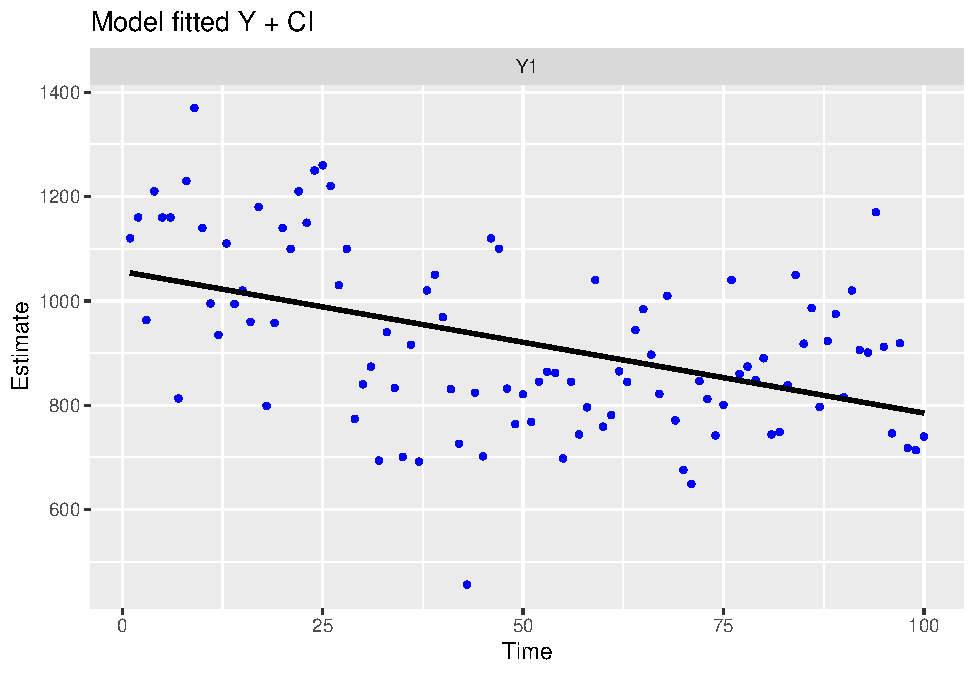
\includegraphics[width=0.8\linewidth]{MARSS_Manual_files/figure-latex/quick-unis-linear-level-plot-1} \end{center}

\hypertarget{stochastic-level-model}{%
\section{Stochastic level model}\label{stochastic-level-model}}

We will now model the average river flow at year \(t\) as a random walk, specifically an autoregressive process which means that average river flow at year \(t\) is a function of average river flow in year \(t-1\).

\begin{equation}
\begin{gathered}
x_t = x_{t-1}+w_t \text{ where } w_t \sim \,\text{N}(0,q) \\
y_t = x_t+v_t \text{ where } v_t \sim \,\text{N}(0,r)  \\
x_0 = \pi 
\end{gathered}   
(\#eq:short.stoch.level.model)
\end{equation}

With all the MARSS parameters shown, the model is:
\begin{equation}
\begin{gathered}
x_t = 1 \times x_{t-1}+ 0 + w_t    \text{ where } w_t \sim \,\text{N}(0,q) \\
y_t = 1 \times x_t + 0 + v_t \text{ where } v_t \sim \,\text{N}(0,r)  \\
x_0 = \pi 
 \end{gathered}   
(\#eq:short.stoch.level.model2)
\end{equation}

The model is specified as a list as follows. We can use the BFGS algorithm to `polish' off the fit and get closer to the MLE. Why not just start with BFGS? First, it happens to take a long long time to fit and more importantly, the BFGS algorith is sensitive to starting conditions and can catostrophically fail. In this case, it is slow but works fine. For some models, it does work better (faster and stable), but using the EM algorithm to get decent starting conditions for the BFGS algorithm is a common fitting strategy.

\begin{Shaded}
\begin{Highlighting}[]
\NormalTok{mod.list =}\StringTok{ }\KeywordTok{list}\NormalTok{(}\DataTypeTok{Z =} \KeywordTok{matrix}\NormalTok{(}\DecValTok{1}\NormalTok{), }\DataTypeTok{A =} \KeywordTok{matrix}\NormalTok{(}\DecValTok{0}\NormalTok{), }\DataTypeTok{R =} \KeywordTok{matrix}\NormalTok{(}\StringTok{"r"}\NormalTok{), }
    \DataTypeTok{B =} \KeywordTok{matrix}\NormalTok{(}\DecValTok{1}\NormalTok{), }\DataTypeTok{U =} \KeywordTok{matrix}\NormalTok{(}\DecValTok{0}\NormalTok{), }\DataTypeTok{Q =} \KeywordTok{matrix}\NormalTok{(}\StringTok{"q"}\NormalTok{), }\DataTypeTok{x0 =} \KeywordTok{matrix}\NormalTok{(}\StringTok{"pi"}\NormalTok{))}
\NormalTok{fit1 <-}\StringTok{ }\KeywordTok{MARSS}\NormalTok{(nile, }\DataTypeTok{model =}\NormalTok{ mod.list, }\DataTypeTok{silent =} \OtherTok{TRUE}\NormalTok{)}
\NormalTok{fit2 <-}\StringTok{ }\KeywordTok{MARSS}\NormalTok{(nile, }\DataTypeTok{model =}\NormalTok{ mod.list, }\DataTypeTok{inits =}\NormalTok{ fit1, }\DataTypeTok{method =} \StringTok{"BFGS"}\NormalTok{)}
\end{Highlighting}
\end{Shaded}

\begin{verbatim}
Success! Converged in 12 iterations.
Function MARSSkfas used for likelihood calculation.

MARSS fit is
Estimation method: BFGS 
Estimation converged in 12 iterations. 
Log-likelihood: -637.7451 
AIC: 1281.49   AICc: 1281.74   
 
      Estimate
R.r      15337
Q.q       1218
x0.pi     1112
Initial states (x0) defined at t=0

Standard errors have not been calculated. 
Use MARSSparamCIs to compute CIs and bias estimates.
\end{verbatim}

\begin{Shaded}
\begin{Highlighting}[]
\NormalTok{ggplot2}\OperatorTok{::}\KeywordTok{autoplot}\NormalTok{(fit2, }\DataTypeTok{plot.type =} \StringTok{"observations"}\NormalTok{)}
\end{Highlighting}
\end{Shaded}

\begin{center}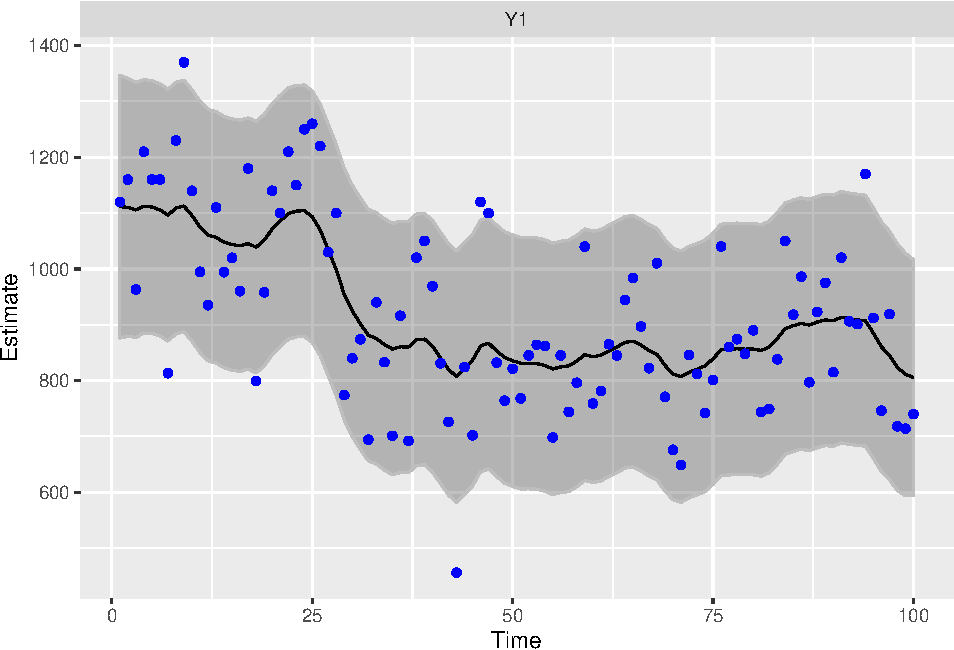
\includegraphics[width=0.8\linewidth]{MARSS_Manual_files/figure-latex/quick-unis-stoch-level-plot-1} \end{center}

This is the same model fit in \citet[p. 148]{Koopmanetal1998} except that we estimate \(x_1\) as parameter rather than specifying \(x_1\) via a diffuse prior\index{prior!diffuse}. As a result, the log-likelihood value and \(\mathbf{R}\) and \(\mathbf{Q}\) are a little different than in \citet{Koopmanetal1998}.

We can fit the Koopman model with \texttt{stats::StructTS()}. The estimates are slightly different since the initial conditions are treated differently.

\begin{Shaded}
\begin{Highlighting}[]
\NormalTok{fit.ts <-}\StringTok{ }\NormalTok{stats}\OperatorTok{::}\KeywordTok{StructTS}\NormalTok{(nile, }\DataTypeTok{type =} \StringTok{"level"}\NormalTok{)}
\NormalTok{fit.ts}
\end{Highlighting}
\end{Shaded}

\begin{verbatim}

Call:
stats::StructTS(x = nile, type = "level")

Variances:
  level  epsilon  
   1469    15099  
\end{verbatim}

The fitted values returned by \texttt{fitted()} applied to a \textbf{StructTS} object are different than that returned by \texttt{fitted()} applied to a \textbf{marssMLE} object. The former returns \(\hat{y}\) conditioned on the data up to time \(t\), while the latter returns the \(\hat{y}\) conditioned on all the data. If you want to compare use:

\begin{Shaded}
\begin{Highlighting}[]
\KeywordTok{plot}\NormalTok{(nile, }\DataTypeTok{type =} \StringTok{"p"}\NormalTok{, }\DataTypeTok{pch =} \DecValTok{16}\NormalTok{, }\DataTypeTok{col =} \StringTok{"blue"}\NormalTok{)}
\KeywordTok{lines}\NormalTok{(}\KeywordTok{fitted}\NormalTok{(fit.ts), }\DataTypeTok{col =} \StringTok{"black"}\NormalTok{, }\DataTypeTok{lwd =} \DecValTok{3}\NormalTok{)}
\KeywordTok{lines}\NormalTok{(}\KeywordTok{MARSSkfss}\NormalTok{(fit2)}\OperatorTok{$}\NormalTok{xtt[}\DecValTok{1}\NormalTok{, ], }\DataTypeTok{col =} \StringTok{"red"}\NormalTok{, }\DataTypeTok{lwd =} \DecValTok{1}\NormalTok{)}
\end{Highlighting}
\end{Shaded}

\begin{center}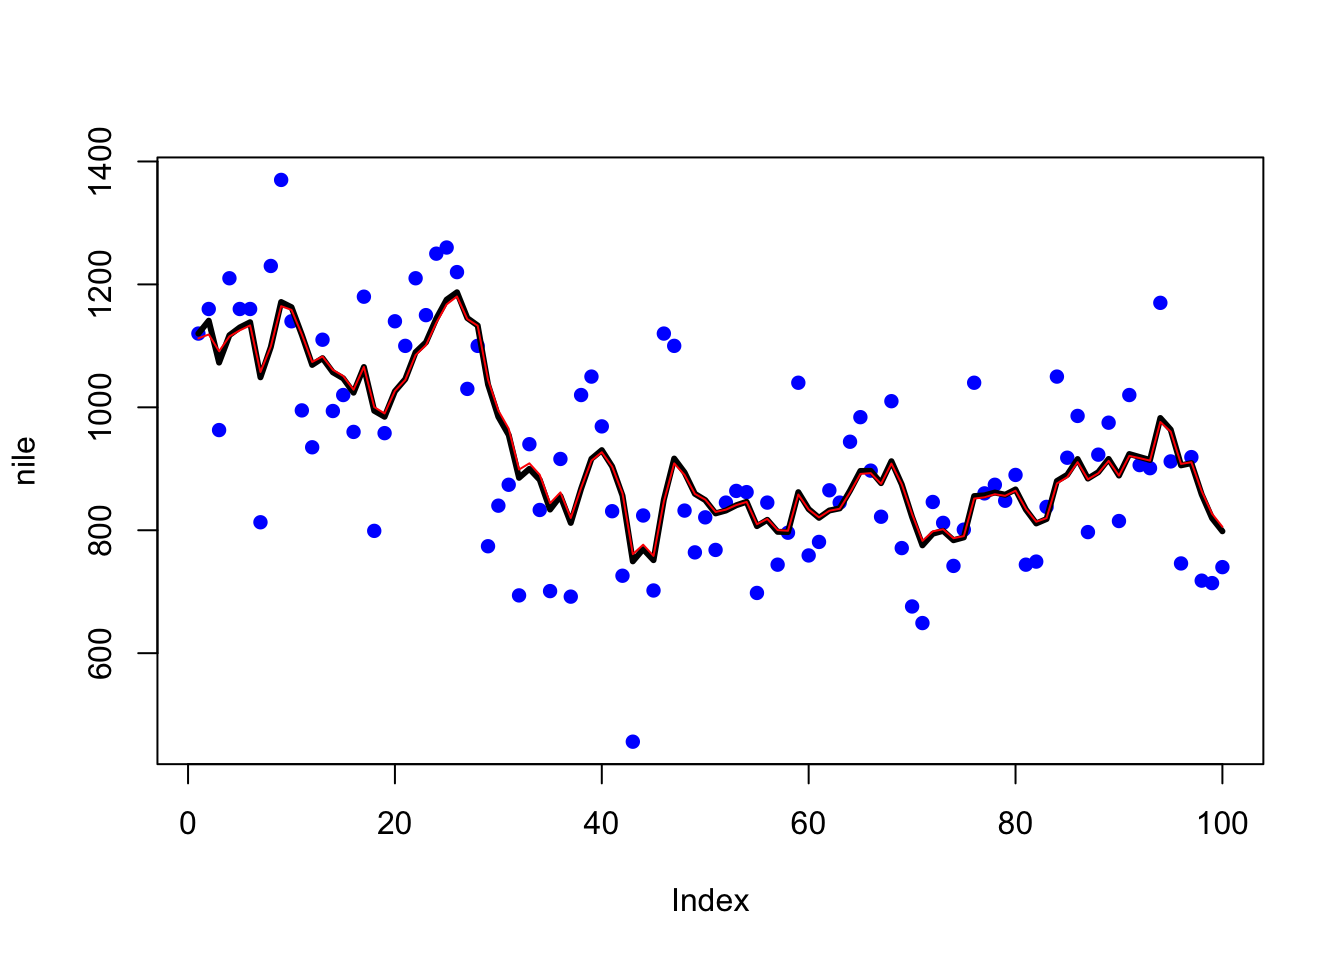
\includegraphics[width=0.8\linewidth]{MARSS_Manual_files/figure-latex/quick-unis-stoch-level-StructTS-plot-1} \end{center}

The black line is the \texttt{StrucTS()} fit and the red line is the equivalent \texttt{MARSS()} fit.

\hypertarget{stochastic-slope-model}{%
\section{Stochastic slope model}\label{stochastic-slope-model}}

We can also model the \(\beta\) as a random walk:

\begin{equation}
\begin{gathered}
\beta_t = \beta_{t-1}+w_t \text{ where } w_t \sim \,\text{N}(0,q) \\
y_t = a + \beta_t*t + v_t \text{ where } v_t \sim \,\text{N}(0,r)  \\
x_0 = \pi 
\end{gathered}   
(\#eq:short.stoch.levelslope.model)
\end{equation}

The \(\beta_t\) is model with \(x_t\). With all the MARSS parameters shown, the model is:
\begin{equation}
\begin{gathered}
x_t = 1 \times x_{t-1}+ 0 + w_t    \text{ where } w_t \sim \,\text{N}(0,q) \\
y_t = t \times x_t + a + v_t \text{ where } v_t \sim \,\text{N}(0,r)  \\
x_0 = \pi 
 \end{gathered}   
(\#eq:short.stoch.slope.model)
\end{equation}
The trick here is to recognize that \(\mathbf{Z}_t\), the matrix in front of \(\mathbf{x}_t\) in the \(\mathbf{y}_t\) equation, can be time-varying and can be fixed. In a time-varying matrix in \textbf{MARSS}, the time element is in the 3rd dimension. We are going to fix \(\mathbf{Z}[1,1,t] = t\), where \(t\) is \texttt{year-mean(year)}. \(\mathbf{Z}\) is a \(1 \times 1 \times 100\) array. Demeaning the covariate stablizes the fitting. Try without demeaning to see the difference.

The model is specified as a list as follows.

\begin{Shaded}
\begin{Highlighting}[]
\NormalTok{Z <-}\StringTok{ }\KeywordTok{array}\NormalTok{(}\DecValTok{0}\NormalTok{, }\DataTypeTok{dim =} \KeywordTok{c}\NormalTok{(}\DecValTok{1}\NormalTok{, }\DecValTok{1}\NormalTok{, }\KeywordTok{length}\NormalTok{(nile)))}
\NormalTok{Z[}\DecValTok{1}\NormalTok{, }\DecValTok{1}\NormalTok{, ] <-}\StringTok{ }\NormalTok{year }\OperatorTok{-}\StringTok{ }\KeywordTok{mean}\NormalTok{(year)}
\NormalTok{mod.list =}\StringTok{ }\KeywordTok{list}\NormalTok{(}\DataTypeTok{Z =}\NormalTok{ Z, }\DataTypeTok{A =} \KeywordTok{matrix}\NormalTok{(}\StringTok{"a"}\NormalTok{), }\DataTypeTok{R =} \KeywordTok{matrix}\NormalTok{(}\StringTok{"r"}\NormalTok{), }\DataTypeTok{B =} \KeywordTok{matrix}\NormalTok{(}\DecValTok{1}\NormalTok{), }
    \DataTypeTok{U =} \KeywordTok{matrix}\NormalTok{(}\DecValTok{0}\NormalTok{), }\DataTypeTok{Q =} \KeywordTok{matrix}\NormalTok{(}\StringTok{"q"}\NormalTok{), }\DataTypeTok{x0 =} \KeywordTok{matrix}\NormalTok{(}\StringTok{"pi"}\NormalTok{))}
\NormalTok{fit1 <-}\StringTok{ }\KeywordTok{MARSS}\NormalTok{(nile, }\DataTypeTok{model =}\NormalTok{ mod.list, }\DataTypeTok{silent =} \OtherTok{TRUE}\NormalTok{)}
\NormalTok{fit2 <-}\StringTok{ }\KeywordTok{MARSS}\NormalTok{(nile, }\DataTypeTok{model =}\NormalTok{ mod.list, }\DataTypeTok{inits =}\NormalTok{ fit1, }\DataTypeTok{method =} \StringTok{"BFGS"}\NormalTok{)}
\end{Highlighting}
\end{Shaded}

\begin{verbatim}
Success! Converged in 13 iterations.
Function MARSSkfas used for likelihood calculation.

MARSS fit is
Estimation method: BFGS 
Estimation converged in 13 iterations. 
Log-likelihood: -636.6226 
AIC: 1281.245   AICc: 1281.666   
 
       Estimate
A.a     836.164
R.r   16835.484
Q.q       0.749
x0.pi    -5.905
Initial states (x0) defined at t=0

Standard errors have not been calculated. 
Use MARSSparamCIs to compute CIs and bias estimates.
\end{verbatim}

\begin{Shaded}
\begin{Highlighting}[]
\NormalTok{ggplot2}\OperatorTok{::}\KeywordTok{autoplot}\NormalTok{(fit2, }\DataTypeTok{plot.type =} \StringTok{"observations"}\NormalTok{)}
\end{Highlighting}
\end{Shaded}

\begin{center}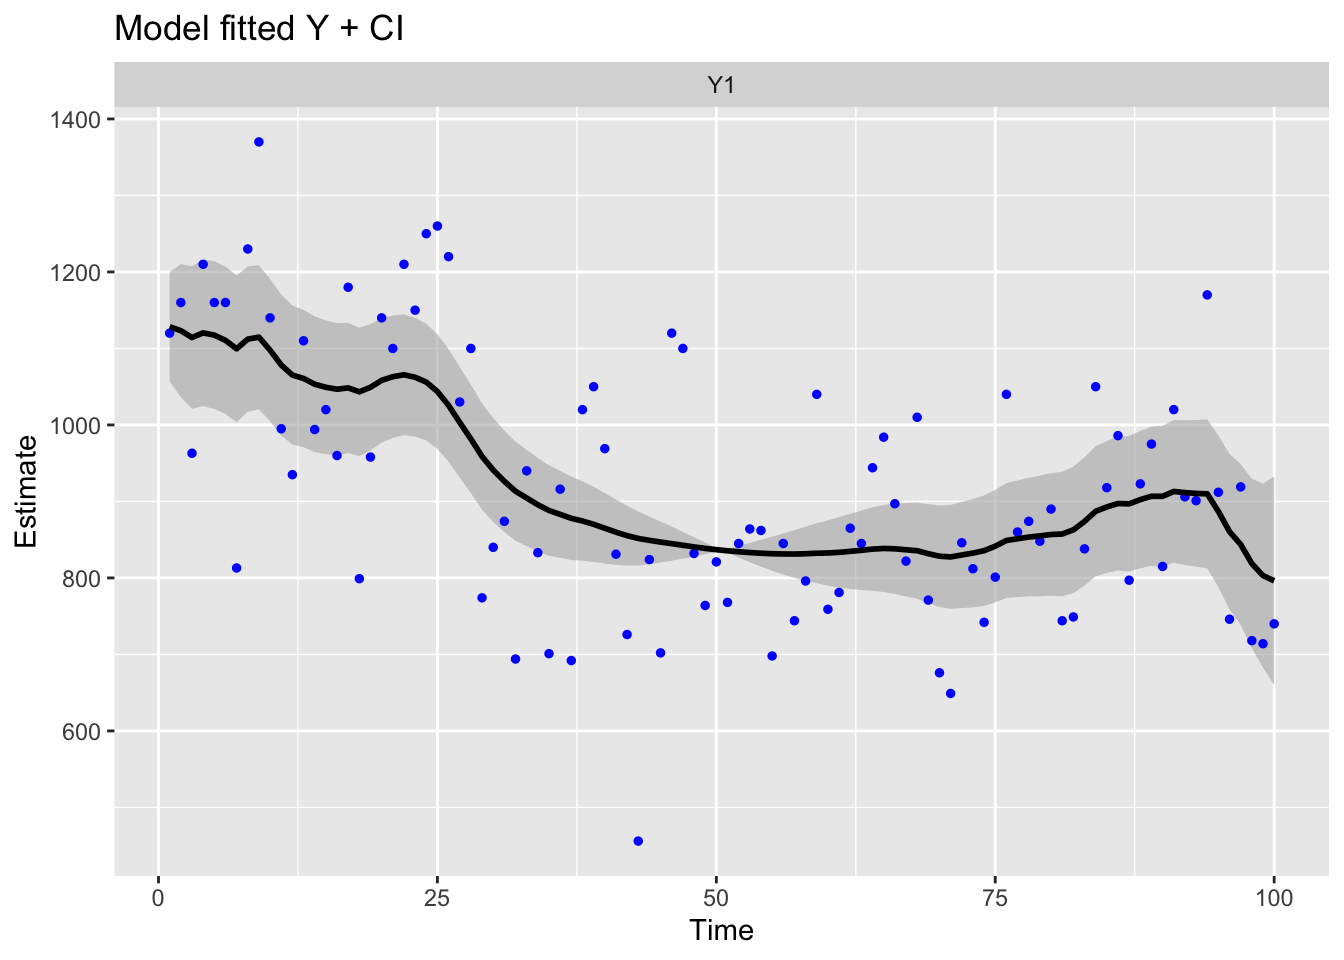
\includegraphics[width=0.8\linewidth]{MARSS_Manual_files/figure-latex/quick-unis-stoch-slope-plot-1} \end{center}

\hypertarget{part3}{%
\chapter*{Part 3. Outputs}\label{part3}}


Part 3 discusses how to get outputs from \textbf{MARSS} fitted objects. Specifically:

\begin{itemize}
\tightlist
\item
  Estimated states
\item
  Kalman filter and smoother output
\item
  Residuals
\item
  Confidence intervals
\item
  Predictions
\item
  Bootstrap resamples: parametric and innovations
\item
  Simulated data
\end{itemize}

\hypertarget{marss-outputs}{%
\chapter{MARSS outputs}\label{marss-outputs}}

MARSS models are used in many different ways and different users will want different types of output. Some users will want the parameter estimates while others want the smoothed states and others want to use MARSS models to interpolate missing values and want the expected values of missing data.

The best way to find out how to get output is to type \texttt{?print.MARSS} at the command line after installing the \textbf{MARSS} package. The print help page discusses how to get parameter estimates in different forms, the smoothed and filtered states, all the Kalman filter and smoother output, all the expectations of y (missing data), confidence intervals and bias estimates for the parameters,
and standard errors of the states. If you are looking only for Kalman filter and smoother output, see the relevant section in Chapter \ref{chap:algorithms} and see the help page for the \texttt{MARSSkf()} function (type \texttt{?MARSSkf} at the ,\textbf{R} command line).

You might also want to look at the \texttt{augment()}, \texttt{tidy()} and \texttt{glance()} functions which will summarize commonly needed output from a MARSS model fit. Type \texttt{?augment.marssMLE} at the command line to see examples. These functions work as they do in the \textbf{broom} R package.

\hypertarget{marss-residuals}{%
\chapter{MARSS Residuals}\label{marss-residuals}}

\hypertarget{confidence-intervals}{%
\chapter{Confidence Intervals}\label{confidence-intervals}}

\hypertarget{predictions}{%
\chapter{Predictions}\label{predictions}}

\hypertarget{part4}{%
\chapter*{Part 4. Tips and Tricks}\label{part4}}


Part 4 discusses troubleshooting, error messages, and tips to get MARSS models to fit quicker and better.

\hypertarget{troubleshooting}{%
\chapter{Troubleshooting}\label{troubleshooting}}

\index{troubleshooting}Numerical errors due to ill-conditioned matrices are not uncommon when fitting MARSS models\index{errors!ill-conditioned}\index{troubleshooting!ill-conditioning}\index{likelihood!troubleshooting}. The Kalman and EM algorithms need inverses of matrices. If those matrices become ill-conditioned, for example all elements are close to the same value, then the algorithm becomes unstable. Warning messages will be printed if the algorithms are becoming unstable\index{troubleshooting!numerical instability} and you can set \texttt{control\$trace=1}, to see details of where the algorithm is becoming unstable. Whenever possible, you should avoid using shared \(\boldsymbol{\pi}\) values in your model\footnote{An example of a $\boldsymbol{\pi}$ with shared values is $\boldsymbol{\pi}=\bigl[\begin{smallmatrix} a\\a\\a \end{smallmatrix} \bigr]$.}. The way our algorithm deals with \(\boldsymbol{\Lambda}\) tends to make this case unstable, especially if \(\mathbf{R}\) is not diagonal. In general, estimation of a non-diagonal \(\mathbf{R}\) is more difficult, more prone to ill-conditioning, and more data-hungry.

You may also see non-convergence warnings, especially if your MLE model turns out to be degenerate\index{errors!degenerate}\index{troubleshooting!degenerate}\index{troubleshooting!non-convergence}. This means that one of the elements on the diagonal of your \(\mathbf{Q}\) or \(\mathbf{R}\) matrix are going to zero (are degenerate). It will take the EM algorithm forever to get to zero. BFGS will have the same problem, although it will often get a bit closer to the degenerate solution. If you are using \texttt{method="kem"}, MARSS will warn you if it looks like the solution is degenerate. If you use \texttt{control=list(allow.degen=TRUE)}, the EM algorithm will attempt to set the degenerate variances to zero (instead of trying to get to zero using an infinite number of iterations). However, if one of the variances is going to zero, first think about why this is happening. This is typically caused by one of three problems: 1) you made a mistake in inputting your data, e.g.~used -99 as the missing value in your data but did not replace these with NAs before passing to MARSS, 2) your data are not sufficient to estimate multiple variances or 3) your data are inconsistent with the model you are trying fit.

The algorithms in the \textbf{MARSS} package are designed for cases where the \(\mathbf{Q}\) and \(\mathbf{R}\) diagonals are all non-minuscule. For example, the EM update equation for \(\mathbf{u}\) will grind to a halt (not update \(\mathbf{u}\)) if \(\mathbf{Q}\) is tiny (like 1E-7). Conversely, the BFGS equations are likely to miss the maximum-likelihood when \(\mathbf{R}\) is tiny because then the likelihood surface becomes hyper-sensitive to \(\boldsymbol{\pi}\). The solution is to use the degenerate likelihood function for the likelihood calculation and the EM update equations. \textbf{MARSS} will implement this automatically when \(\mathbf{Q}\) or \(\mathbf{R}\) diagonal elements are set to zero and will try setting \(\mathbf{Q}\) and \(\mathbf{R}\) terms to zero automatically if \texttt{control\$allow.degen=TRUE}.

One odd case can occur when \(\mathbf{R}\) goes to zero (a matrix of zeros), but you are estimating \(\boldsymbol{\pi}\). If \texttt{model\$tinitx=1}, then \(\boldsymbol{\pi}=\mathbf{x}_1^0\) and \(\mathbf{y}_1-\mathbf{Z}\mathbf{x}_1^0\) can go to 0 as well as \(\,\text{var}(\mathbf{y}_1-\mathbf{Z}\mathbf{x}_1^0)\) by driving \(\mathbf{R}\) to zero. But as this happens, the log-likelihood associated with \(\mathbf{y}_1\) will go (correctly) to infinity and thus the log-likelihood goes to infinity. But if you set \(\mathbf{R}=0\), the log-likelihood will be finite. The reason is that \(\mathbf{R} \approx 0\) and \(\mathbf{R}=0\) specify different likelihoods associated with \(\mathbf{y}_1-\mathbf{Z}\mathbf{x}_1^0\). With \(\mathbf{R}=0\), \(\mathbf{y}_1-\mathbf{Z}\mathbf{x}_1^0\) does not have a distribution; it is just a fixed value. So there is no likelihood to go to infinity. If some elements of the diagonal of \(\mathbf{R}\) are going to zero, you should be suspect of the parameter estimates. Sometimes the structure of your data, e.g.~one data value followed by a long string of missing values, is causing an odd spike in the likelihood at \(\mathbf{R} \approx 0\). Try manually setting \(\mathbf{R}\) equal to zero to get the correct log-likelihood\footnote{The likelihood returned when $\mathbf{R} \approx 0$ is not incorrect.  It is just not the likelihood that you probably want.  You want the likelihood where the $\mathbf{R}$ term is dropped because it is zero.}.

\hypertarget{em-algorithm}{%
\chapter{EM algorithm}\label{em-algorithm}}

The \textbf{MARSS} package fits models via maximum likelihood. The MARSS package is unusual among packages for fitting MARSS models in that fitting is performed via a constrained EM algorithm \citep{Holmes2010} based on a vectorized form of Equation \ref{eqn:marss} (See Chapter \ref{chap:algorithms} for the vectorized form used in the algorithm). Although fitting via the BFGS algorithm is also provided using \texttt{method="BFGS"} and the optim function in ,\textbf{R}, the examples in this guide use the EM algorithm primarily because it gives robust estimation for datasets replete with missing values and for high-dimensional models with various constraints. However, there are many models/datasets where BFGS is faster and we typically try both for problems. The EM algorithm is also often used to provide initial conditions for the BFGS algorithm (or an MCMC routine) in order to improve the performance of those algorithms. In addition to the main model fitting function, the MARSS package supplies functions for bootstrap and approximate confidence intervals, parametric and non-parametric bootstrapping, model selection (AIC and bootstrap AIC), simulation, and bootstrap bias correction.

\hypertarget{important-notes-about-the-algorithms}{%
\section{Important notes about the algorithms}\label{important-notes-about-the-algorithms}}

Specification of a properly constrained model with a unique solution is the responsibility of the user because MARSS has no way to tell if you have specified an insufficiently constrained model---with correspondingly an infinite number of solutions.
How do you know if the model is properly constrained? If you are using a MARSS model form that is widely used, then you can probably assume that it is properly constrained. If you go to papers where someone developed the model or method, the issue of constraints necessary to ensure ``identifiability'' will likely be addressed if it is an issue. Are you fitting novel MARSS models? Then you will need to do some study on identifiability in this class of models using textbooks (Appendix \ref{chap:SSreferences}). Often textbooks do not address identifiability explicitly. Rather it is addressed implicitly by only showing a model constructed in such a way that it is identifiable. In our work, if we suspect identification problems, we will often first do a Bayesian analysis with flat priors and look for oddities in the posteriors, such as ridges, plateaus or bimodality.

All the EM code in the \textbf{MARSS} package is currently in native ,\textbf{R}. Thus the model fitting is slow. The classic Kalman filter/smoother algorithm, as shown in \citet[p. 331-335]{ShumwayStoffer2006}, is based on the original smoother presented in \citet{Rauch1963}. This Kalman filter is provided in function \texttt{MARSSkfss()}, but the default Kalman filter and smoother used in the \textbf{MARSS} package is based on the algorithm in \citet{KohnAnsley1989} and papers by Koopman et al.~This Kalman filter and smoother is provided in the \textbf{KFAS} package (Helske 2012). Table 2 in \citet{Koopman1993} indicates that the classic algorithm is 40-100 times slower than the algorithm given in \citet{KohnAnsley1989}, \citet{Koopman1993}, and \citet{Koopmanetal1998}. The MARSS package function \texttt{MARSSkfas()} provides a translator between the model objects in MARSS and those in \textbf{KFAS} so that the \textbf{KFAS} functions can be used. \texttt{MARSSkfas()} also includes a lag-one covariance smoother algorithm as this is not output by the \textbf{KFAS} functions, and it provides proper formulation of the priors so that one can use the \textbf{KFAS} functions when the prior on the states is set at \(t=0\) instead of \(t=1\). Simply off-setting your data to start at t=2 and sending that value to \(t_{init}=1\) in the \textbf{KFAS} Kalman filter would not be mathematically correct!

EM algorithms will quickly get in the vicinity of the maximum likelihood, but the final approach to the maximum is generally slow relative to quasi-Newton methods. On the flip side, EM algorithms are quite robust to initial conditions choices and can be extremely fast at getting close to the MLE values for high-dimensional models. The \textbf{MARSS} package also allows one to use the BFGS method to fit MARSS models, thus one can use an EM algorithm to ``get close'' and then the BFGS algorithm to polish off the estimate. Restricted maximum-likelihood algorithms\index{estimation!REML} are also available for AR(1) state-space models, both univariate \citep{Staplesetal2004} and multivariate \citep{HinrichsenHolmes2009}. REML can give parameter estimates with lower variance than plain maximum-likelihood algorithms. However, the algorithms for REML when there are missing values are not currently available (although that will probably change in the near future). Another maximum-likelihood method is data-cloning which adapts MCMC algorithms used in Bayesian analysis for maximum-likelihood estimation \citep{Leleetal2007}.

Missing values\index{missing values} are seamlessly accommodated with the \textbf{MARSS} package. Simply specify missing data with NAs. The likelihood computations are exact and will deal appropriately with missing values. However, no innovations, referring to the non-parametric bootstrap developed by Stoffer and Wall (1991), bootstrapping can be done if there are missing values. Instead parametric bootstrapping must be used.

You should be aware that maximum-likelihood estimates of variance in MARSS models are fundamentally biased, regardless of the algorithm used. This bias is more severe when one or the other of \(\mathbf{R}\) or \(\mathbf{Q}\) is very small, and the bias does not go to zero as sample size goes to infinity. The bias arises because variance is constrained to be positive. Thus if \(\mathbf{R}\) or \(\mathbf{Q}\) is essentially zero, the mean estimate will not be zero and thus the estimate will be biased high while the corresponding bias of the other variance will be biased low. You can generate unbiased variance estimates using a bootstrap estimate of the bias. The function \texttt{MARSSparamCIs()}\index{functions!MARSSparamCIs} will do this. However be aware that adding an estimated bias to a parameter estimate will lead to an increase in the variance of your parameter estimate. The amount of variance added will depend on sample size.

You should also be aware that mis-specification of the prior on the initial states (\(\boldsymbol{\pi}\) and \(\boldsymbol{\Lambda}\)) can have catastrophic effects on your parameter estimates if your prior conflicts with the distribution of the initial states implied by the MARSS model\index{prior!troubleshooting}. These effects can be very difficult to detect because the model will appear to be well-fitted. Unless you have a good idea of what the parameters should be, you might not realize that your prior conflicts.

The most common problems we have found with priors on \(\mathbf{x}_0\) are the following. Problem 1) The correlation structure in \(\boldsymbol{\Lambda}\) (whether the prior is diffuse or not) does not match the correlation structure in \(\mathbf{x}_0\) implied by your model. For example, you specify a diagonal \(\boldsymbol{\Lambda}\) (independent states), but the implied distribution has correlations. Problem 2) The correlation structure in \(\boldsymbol{\Lambda}\) does not match the structure in \(\mathbf{x}_0\) implied by constraints you placed on \(\boldsymbol{\pi}\). For example, you specify that all values in \(\boldsymbol{\pi}\) are shared, yet you specify that \(\boldsymbol{\Lambda}\) is diagonal (independent).

Unfortunately, using a diffuse prior does not help with these two problems because the diffuse prior still has a correlation structure and can still conflict with the implied correlation in \(\mathbf{x}_0\). One way to get around these problems is to set \(\boldsymbol{\Lambda}\)=0 (a \(m \times m\) matrix of zeros) and estimate \(\boldsymbol{\pi} \equiv \mathbf{x}_0\) only. Now \(\boldsymbol{\pi}\) is a fixed but unknown (estimated) parameter, not the mean of a distribution. In this case, \(\boldsymbol{\Lambda}\) does not exist in your model and there is no conflict with the model.\\
Be aware however that estimating \(\boldsymbol{\pi}\) as a parameter is not always robust. If you specify that \(\boldsymbol{\Lambda}\)=0 and specify that \(\boldsymbol{\pi}\) corresponds to \(\mathbf{x}_0\), but your model ``explodes'' when run backwards in time, you cannot estimate \(\boldsymbol{\pi}\) because you cannot get a good estimate of \(\mathbf{x}_0\). Sometimes this can be avoided by specifying that \(\boldsymbol{\pi}\) corresponds to \(\mathbf{x}_1\) so that it can be constrained by the data \(\mathbf{y}_1\).

In summary, if the implied correlation structure of your initial states is independent (diagonal variance-covariance matrix), you should generally be ok with a diagonal and high variance prior or with treating the initial states as parameters (with \(\boldsymbol{\Lambda}=0\)). But if your initial states have an implied correlation structure that is not independent, then proceed with caution. `With caution' means that you should assume you have problems and test how your model fits with simulated data.

\hypertarget{state-space-form-of-armapq-models}{%
\section{State-space form of ARMA(p,q) models}\label{state-space-form-of-armapq-models}}

There is a large class of models in the statistical finance literature that have the form
\begin{equation*}
\begin{gathered}
\mathbf{x}_{t+1} = \mathbf{B}\mathbf{x}_t + \boldsymbol{\Gamma}\boldsymbol{\eta}_t\\
\mathbf{y}_t = \mathbf{Z}\mathbf{x}_t  + \boldsymbol{\eta}_t\\
\end{gathered}
\end{equation*}
For example, ARMA(p,q) models can be written in this form. The MARSS model framework in this package will not allow you to write models in that form. You can put the \(\boldsymbol{\eta}_t\) into the \(\mathbf{x}_t\) vector and set \(\mathbf{R}=0\) to make models of this form using the MARSS form, but the EM algorithm in the MARSS package won't let you estimate parameters because the parameters will drop out of the full likelihood being maximized in the algorithm. You can try using BFGS by passing in the \texttt{method} argument to the MARSS() call.

\hypertarget{other-related-packages}{%
\chapter{Other related packages}\label{other-related-packages}}

Packages that will do Kalman filtering and smoothing are many, but packages that estimate the parameters in a MARSS model, especially constrained MARSS models, are much less common. The following are those with which we are familiar, however there are certainly more packages for estimating MARSS models in engineering and economics of which we are unfamiliar. The \textbf{MARSS} package is unusual in that it uses an EM algorithm for maximizing the likelihood as opposed to a Newton-esque method (e.g.~BFGS). The package is also unusual in that it allows you to specify the initial conditions at \(t=0\) or \(t=1\), allows degenerate models (with some of the diagonal elements of \(\mathbf{R}\) or \(\mathbf{Q}\) equal to zero). Lastly, model specification in the \textbf{MARSS} package has a one-to-one relationship between the model list in \texttt{MARSS()} and the model as you would write it on paper as a matrix equation. This makes the learning curve a bit less steep. However, the \textbf{MARSS} package has not been optimized for speed and probably will be really slow if you have time-series data with a lot of time points.

\begin{description}
    \item[atsar] \href{https://nwfsc-timeseries.github.io/atsar/}{atsar} is an \,\textbf{R} package we wrote for fitting MARSS models using STAN.  It allows fast and flexible fitting of MARSS models in a Bayesian framework.  Our book from our time-series class has example applications \href{https://nwfsc-timeseries.github.io/atsa-labs/}{Applied Time-Series Analysis for Fisheries and Environmental Sciences}.
  \item[stats] The **stats** package (part of base R) has functions for fitting univariate structural time series models (MARSS models with a univariate $y$).  Read the help file at `?StructTS`. The Kalman filter and smoother functions are described here: `?KalmanLike`.
    \item[DLM] \href{https://cran.r-project.org/package=dlm}{DLM} is an \,\textbf{R} package for fitting MARSS models.  Our impression is that it is mainly Bayesian focused but it does allow MLE estimation via the `optim()` function.  It has a book, *Dynamic Linear Models* with \,\textbf{R}  by Petris et al., which has many examples of how to write MARSS models for different applications.
    \item[sspir] \href{https://cran.r-project.org/package=sspir}{sspir} an \,\textbf{R} package for fitting ARSS (univariate) models with Gaussian, Poisson and binomial error distributions.  
    \item[dse] \href{https://cran.r-project.org/package=dse}{dse} (Dynamic Systems Estimation) is an \,\textbf{R} package for multivariate Gaussian state-space models with a focus on ARMA models.
    \item[SsfPack] \href{http://www.ssfpack.com/}{SsfPack} is a package for Ox/Splus that fits constrained multivariate Gaussian state-space models using mainly (it seems) the BFGS algorithm but the newer versions support other types of maximization.  **SsfPack** is very flexible and written in C to be fast.  It has been used extensively on statistical finance problems and is optimized for dealing with large (financial) data sets.  It is used and documented in *Time Series Analysis by State Space Methods* by Durbin and Koopman, *An Introduction to State Space Time Series Analysis* by Commandeur and Koopman, and *Statistical Algorithms for Models in State Space Form: SsfPack 3.0*, by Koopman, Shephard, and Doornik.
    \item[Brodgar] The Brodgar software was developed by Alain Zuur to do (among many other things) dynamic factor analysis, which involves a special type of MARSS model.  The methods and many example analyses are given in *Analyzing Ecological Data* by Zuur, Ieno and Smith.  This is the one package that we are aware of that also uses an EM algorithm for parameter estimation.
    \item[eViews] **eViews** is a commercial economics software that will estimate at least some types of MARSS models.
    \item[KFAS] The \href{https://cran.r-project.org/package=KFAS}{KFAS} \,\textbf{R} package provides a fast Kalman filter and smoother.  Examples in the package show how to estimate MARSS models using the **KFAS** functions and \,\textbf{R}'s `optim()` function.   The **MARSS** package uses the filter and smoother functions from the **KFAS** package.
        \item[S+FinMetrics] \href{http://faculty.washington.edu/ezivot/MFTS2ndEditionFinMetrics.htm}{S+FinMetrics} is a S-plus module for fitting MAR models, which are called vector autoregressive (VAR) models in the economics and finance literature.  It has some support for state-space VAR models, though we haven't used it so are not sure which parameters it allows you to estimate.  It was developed by Andrew Bruce, Doug Martin, Jiahui Wang, and Eric Zivot, and it has a book associated with it: *Modeling Financial Time Series with S-plus* by Eric Zivot and Jiahui Wang.
        \item[kftrack] The \href{https://github.com/positioning/kalmanfilter/wiki}{kftrack} \,\textbf{R} package provides a suite of functions specialized for fitting MARSS models to animal tracking data.
\end{description}

\bibliography{tex/book.bib,tex/packages.bib}


\end{document}
